\documentclass[titlepage, 11pt]{article}
\usepackage[a4paper, total={6in, 9.5in}]{geometry}
\usepackage{graphicx}
\usepackage{amsmath,amsfonts,amssymb}
\usepackage{listings}
\usepackage{booktabs}
\usepackage[T1]{fontenc}
\usepackage{listings}
\usepackage{color}
\usepackage{minted}
\usepackage{multirow}
\usepackage[colorlinks=true, linkcolor=blue, urlcolor=blue, citecolor=blue, pdfborder={0 0 255}]{hyperref}
\usepackage{colortbl}
\usepackage{url}
\usepackage{xcolor}
\usepackage{caption}
\usepackage{subcaption}
\usepackage{dirtytalk}
\usepackage{multirow}
\usepackage[semicolon, round]{natbib}
\usepackage[ruled]{algorithm2e}
\pdfimageresolution=300
\lstdefinestyle{mystyle}{
    backgroundcolor=\color{white},   
    commentstyle=\color{orange},
    keywordstyle=\color{blue},
    numberstyle=\tiny\color{gray},
    stringstyle=\color{red},
    basicstyle=\footnotesize\ttfamily,
    breakatwhitespace=false,         
    breaklines=true,                 
    captionpos=b,                    
    keepspaces=true,                 
    numbers=left,                    
    numbersep=5pt,                  
    showspaces=false,                
    showstringspaces=false,
    showtabs=false,                  
    tabsize=2
}
\lstset{style=mystyle}
% Define color for the background
\definecolor{lightgray}{HTML}{F0F0F0}
% Define custom command for code block
\newcommand{\mycode}[1]{%
\begin{tcolorbox}[colback=lightgray, boxrule=0pt, arc=0pt, boxsep=0pt, left=0pt, right=0pt, top=0pt, bottom=0pt]%
\texttt{#1}%
\end{tcolorbox}%
}
\newcommand{\floor}[1]{\left\lfloor #1 \right\rfloor}
\newcommand{\ceil}[1]{\left\lceil #1 \right\rceil}
\captionsetup[table]{skip=10pt}
\renewcommand{\vec}[1]{\mathbf{#1}}
\SetKwComment{Comment}{$\triangleright$\ }{}
\definecolor{light-gray}{gray}{0.90}
\newcommand{\code}[1]
{\colorbox{light-gray}{\texttt{#1}}}
\title{\textbf{DiceForge Documentation}}
\author{\textbf{Mathematics Club, IIT Madras}\\\\
Pradyumnan Raghuveeran AE22B009\\\\
Kulkarni Chinmay Ashish EE22B158\\\\
Kailash Gopal D CS22B098\\\\
Advik Kabra CS23B004\\\\
S Kevin Kinsey EP23B027\\\\
Parijat Mukherjee CS23B049\\\\
Madhav Bhardwaj CS23B035\\\\
Navinkumar L EE23B047\\\\
Achintya Raghavan EE23B189\\\\
Astha Chand EE23B013\\\\
D V Anantha Padmanabh ME23B012\\\\
Aditya Sawant CS23B003\\\\
Aditi Vaidya ME23B248\\\\
Shanddhoshkumar Senthilkumar EE23B116}
\date{}
\begin{document}

\maketitle
\newpage

\setcounter{page}{0}
\tableofcontents
\listoffigures
\listoftables
\newpage

\section{Introduction}
DiceForge is a C++ library with the same functionality as Python's random library with more features useful in scientific computing. 
\newline
\newline
DiceForge's functionality can be split into three major sections - pseudo random number generation, sampling probability distributions, and fitting data to standard probability distributions.
\newline
\newline
Blum Blum Shub (BBS), Linear Feedback Shift Register (LFSR), Mersenne Twister (MT), XOR Shift, and Naor-Reingold pseudo-random function are the supported algorithms for generating pseudo random numbers.
All the algorithms can generate:
\begin{itemize}
    \item [(a)] A uniformly selected non-zero 64-bit or 32-bit unsigned integer.
    \item [(b)] A uniformly selected floating point number between 0 and 1
    \item [(c)] A uniformly selected integer between two integers a and b (both inclusive).
    \item [(d)] A uniformly selected float floating point number between two values a and b.
\end{itemize}
On a general note, MT, LFSR and XORShift are suited for generating pseudo-random numbers quickly for fast computation while BBS and Naor Reingold are considerably slow but are more suited for Cryptographic purposes. Although Naor Reingold is Cryptographically safe, the key is fixed in DiceForge's implementation of the same.
\newline
\newline
In addition to the uniform distribution (which is an inbuilt function of the generators themselves), DiceForge supports the generation of samples from Cauchy, Exponential, Gaussian (Normal), Maxwell, Weibull, Bernoulli, Binomial, Geometric, Gibbs, Hypergeometric, Negative-Hypergeometric, and Poisson distributions. A class 'CustomDistribution' is also featured for sampling random variables from user defined distributions for any given valid PDF.
\newline
\newline
Currently, DiceForge supports the fitting of probability density data to the standard continuous probability distributions in section \hyperref[sec:6]{6}.
\newline
\newline
DiceForge also includes a ready-made random number generator \code{Random}, a global instance of the XORShift64 class. Users can run all the functions in section \hyperref[sec:2]{2} on \code{Random} without delving into the object-oriented programming aspects. 
\newline
\newline
For readability and convenience, DiceForge often uses the following predefined datatypes:
\begin{itemize}
    \item 
    \code{int32\_t\, int64\_t\, int128\_t}
    Signed 32-bit, 64-bit, 128-bit integers
    
    \item 
    \code{uint32\_t\, uint64\_t\, uint128\_t}
    Unsigned 32-bit, 64-bit, 128-bit integers
    
    \item 
    \code{real\_t}
    A 64-bit floating point number (double)
    
    \item 
    \code{int\_t}
    A 64-bit signed integer
    
    \item 
    \code{uint\_t}
    A 64-bit unsigned integer 
\end{itemize}

\newpage
\section {Functions of the RNGs}
\label{sec:2}
\subsection{Bookkeeping functions}
\code{void rng.reseed(T seed)}
\newline
\newline
Initializes the RNG with specified seed.
\newline
T is the data type supported by the derived class
\newline
If a is 0, the current system time is used as the seed. Otherwise, the integer a is used directly.


\subsection{Functions to generate integers}
\code{T rng.next()}
\newline
\newline
Generates and returns a uniformly selected random integer of type T (by default, unsigned long long int).
\newline
\newline
\code{T rng.next\_in\_range(T min, T max)}
\newline
\newline
Generates and returns a uniformly selected random integer of type T between min and max (both inclusive).


\subsection{Functions to generate floats}
\code{real\_t rng.next\_unit()}
\newline
\newline
Generates and returns a uniformly selected real number of type real\_t between 0 (inclusive) and 1 (exclusive).
\newline
\newline
\code{real\_t rng.next\_in\_crange(real\_t min, real\_t max)}
\newline
\newline
Generates and returns a uniformly selected random real number of type real\_t between min (inclusive) and max (exclusive).


\subsection{Functions acting on sequences}
\code{auto rng.choice(RandomAccessIterator first, RandomAccessIterator last)}
\newline
\newline
Returns a randomly chosen element from the sequence defined by \code{first} and \code{last}.
\newline
\newline
\code{void rng.shuffle(RandomAccessIterator first, RandomAccessIterator last)}
\newline
\newline
Randomly shuffles the sequence defined by \code{first} and \code{last}, in place.


\newpage
\section{Functions of the Distributions} 
\subsection{Continuous}
\label{sec:3.1}
\code{real\_t dist.expectation()}
\newline
\newline
Returns the theoretically calculated expecation value of the distribution as a floating point number.
\newline
\newline
\code{real\_t dist.variance()}
\newline
\newline
Returns the theoretically calculated variance of the distribution as a floating point number.
\newline
\newline
\code{real\_t dist.minValue()}
\newline
\newline
Returns the theoretical minimum value of the distribution as a floating point number.
\newline
\newline
\code{real\_t dist.maxValue()}
\newline
\newline
Returns the theoretical maximum value of the distribution as a floating point number.
\newline
\newline
\code{real\_t dist.pdf(real\_t x)}
\newline
\newline
Returns (as a floating point number) the probability density of the distribution at a floating point number x.
\newline
\newline
\code{real\_t dist.cdf(real\_t x)}
\newline
\newline
Returns (as a floating point number) the probability of generating a floating point number less than or equal to the floating point number x by the distribution.

\subsection{Discrete}
\label{sec:3.2}
\code{real\_t dist.expectation()}
\newline
\newline
Returns the theoretically calculated expectation value of the distribution as a floating point number.
\newline
\newline
\code{real\_t dist.variance()}
\newline
\newline
Returns the theoretically calculated variance of the distribution as a floating point number.
\newline
\newline
\code{int dist.minValue()}
\newline
\newline
Returns the theoretical minimum value of the distribution as an integer.
\newline
\newline
\code{int dist.maxValue()}
\newline
\newline
Returns the theoretical maximum value of the distribution as an integer.
\newline
\newline
\code{real\_t dist.pmf(int x)}
\newline
\newline
Returns (as a floating point number) the probability of generating the integer x by the distribution.
\newline
\newline
\code{real\_t dist.cdf(int x)}
\newline
\newline
Returns (as a floating point number) the probability of generating an integer less than or equal to the integer x by the distribution.


\newpage
\section{Functions for Fitting Data}

DiceForge also supports fitting a given set of points representing the probability density function of a distribution and fits it to one of the standard \textbf{continuous} distributions enlisted in section \hyperref[sec:6]{6}.

\subsection{Fitting to a Cauchy distribution}
\code{DiceForge::Cauchy fitToCauchy(vector x, vector y, int max\_iter,}
\newline
\code{real\_t epsilon)}
\newline
\newline
Fits the given sample points (x, y=pdf(x)) to a Cauchy distribution using non-linear least squares regression.
\newline\\
Here \code{x} is the list of x coordinates as a \code{std::vector<real\_t>} and \code{y} is the list of the corresponding y coordinates as a \code{std::vector<real\_t>}.\
\code{max\_iter} is the maximum iterations to attempt to fit the data (higher to try for better fits) and \code{epsilon} is the minimum acceptable error tolerance while attempting to fit the data (smaller to try for better fits).\\
\newline
The function returns a \code{DiceForge::Cauchy} distribution fit to the given sample points

\subsection{Fitting to an Exponential distribution}
\code{DiceForge::Exponential fitToExponential(std::vector<real\_t> x, }
\newline
\code{std::vector<real\_t> y, int max\_iter, real\_t epsilon)}
\newline
\newline
Fits the given sample points (x, y=pdf(x)) to an Exponential distribution using a variant of Stochastic Gradient Descent (SGD) with a learning rate that decreases over time. The algorithm takes the natural logarithm of the pdf and optimizes using SGD with the mean square error of the cost function.
\newline\\
Here \code{x} is the list of x coordinates as a \code{std::vector<real\_t>} and \code{y} is the list of the corresponding y coordinates as a \code{std::vector<real\_t>},\
\code{max\_iter} is the maximum iterations to attempt to fit the data and \code{epsilon} is the minimum acceptable error tolerance while attempting to fit the data.
\newline
(defaults:
\code{max\_iter = 10000, epsilon = 1e-6}, optimum value in general cases, change according to requirement)\\
\newline
The function returns a \code{DiceForge::Exponential} distribution fit to the given sample points.
\subsection{Fitting to an Gaussian distribution}
\code{DiceForge::Cauchy fitToGaussian(vector x, vector y, int max\_iter,}
\newline
\code{real\_t epsilon)}
\newline
\newline
Fits the given sample points (x, y=pdf(x)) to a Gaussian distribution using non-linear least squares regression.
\newline\\
Here \code{x} is the list of x coordinates as a \code{std::vector<real\_t>} and \code{y} is the list of the corresponding y coordinates as a \code{std::vector<real\_t>}.\
\code{max\_iter} is the maximum iterations to attempt to fit the data (higher to try for better fits) and \code{epsilon} is the minimum acceptable error tolerance while attempting to fit the data (smaller to try for better fits).\\
\newline
The function returns a \code{DiceForge::Gaussian} distribution fit to the given sample points
\subsection{Fitting to a Maxwell distribution}
\code{DiceForge::Maxwell fitToMaxwell(vector x, vector y, int max\_iter,}
\newline
\code{real\_t epsilon)}
\newline 
\newline
Fits the given sample points (x, y=pdf(x)) to a Maxwell distribution using non-linear least squares regression.
\newline\\
Here \code{x} is the list of x coordinates as a \code{std::vector<real\_t>} and \code{y} is the list of the corresponding y coordinates as a \code{std:vector<real\_t>}.\
\code{max\_iter} is the maximum iterations to attempt to fit the data (higher to try for better fits) and \code{epsilon} is the minimum acceptable error tolerance while attempting to fit the data (smaller to try for better fits).\\
\newline
The function returns a \code{DiceForge::Maxwell} distribution fit to the given sample points.

\subsection{Fitting to a Weibull distribution}
\code{DiceForge::Weibull fitToWeibull(vector x, vector y, int max\_iter,}
\newline
\code{real\_t epsilon)}
\newline 
\newline
Fits the given sample points (x, y=pdf(x)) to a Weibull distribution using non-linear least squares regression.
\newline It approximates the initial guess by calculating CDF and applying regression to find the parameters $\lambda$ and $k$. The regression of CDF method gives very good guess for initial starting point for the Gauss-Newton method, as the CDF of Weibull is a linearizable function. After the guess is found, the non-linear least squares regression is used to approach and fine tune the final parameter values.
\newline\\
Here \code{x} is the list of x coordinates as a \code{std::vector<real\_t>} and \code{y} is the list of the corresponding y coordinates as a \code{std:vector<real\_t>}.\
\code{max\_iter} is the maximum iterations to attempt to fit the data (higher to try for better fits) and \code{epsilon} is the minimum acceptable error tolerance while attempting to fit the data (smaller to try for better fits).\\
\newline
The function returns a \code{DiceForge::Weibull} distribution fit to the given sample points.

\newpage
\section {Generators supported}
\subsection{Linear Feedback Shift Register}
A linear feedback shift register (LFSR) is an algorithm which generates psuedo-random numbers by performing certain linear operations on the seed. The DiceForge library implements a specific type of LFSR called XORshift LFSR, where the linear operation is the exclusive OR. To introduce non-linearity (and thus decrease predictability), the generated number is multiplied with a constant before outputting.

\subsubsection{Algorithm}
\begin{enumerate}
\item Define a function $f_{p, q, r, s}(x)$ over $x \in \mathbb{N}$, such that $f_{p, q, r, s}(x) = ((x >> p) \oplus (x >> q) \oplus (x >> r) \oplus (x >> s)) \mathbin{\&} 1$. This function outputs a single bit, which will be pushed to the MSB.
\item Choose a seed $s (\neq 0)$ and set $x_0 = s$.
\item Choose a constant $M$ and natural numbers $p$, $q$, $r$ and $s$. $p$, $q$, $r$ and $s$ are chosen so as to get the maximum period of the LFSR.
\item Choose the required number of bits, $N$, in the output.
\item Initialise the output $y_0$ to zero.
\item Define a function $g_l (x, b)$ over $x \in \mathbb{N}$ and $b \in \{0, 1\}$, such that $g_l (x, b) = (x >> 1) \& (b << (l - 1))$. Here $l$ is the number of bits in the seed $s$.
\item $b = f_{p, q, r, s}(x_n)$
\newline
$x_{n + 1} = g_l (x_n, b)$
\newline
$y_{n + 1} = 2y_n + (x_{n + 1} \mathbin{\&} 1)$
\item
The sequence of random numbers obtained from the states $\{x_n\}$ is $\{y_{64n} \times M\}$ for $n \in \mathbb{N}$.
\end{enumerate}
DiceForge implements this algorithm with the following values:
\begin{itemize}
    \item $l = 128$.
    \item $M = (2545F4914F6CDD1D)_{16}$.
    \item $\langle p, q, r, s \rangle = \langle 0, 1, 2, 7 \rangle$. This particular tuple gives a cycle length of $2^{128} - 1$, which is the highest possible for a 128-bit seed.
    \item $N = 64$ (for LFSR64) or $32$ (for LFSR32).
\end{itemize}


\subsection{Blum Blum Shub}
The Blum-Blum-Shub  follows a deterministic algorithm to output a sequence that appears to be random. That is, no poly-time algorithm will be able to distinguish between an output sequence of the BBS generator and a truly random sequence with probability significantly greater than 1/2. It is widely used for Cryptographic purposes and the security of BBS generator is as hard as factoring a large composite integer. 

\subsubsection{Algorithm}
\begin{enumerate}
\item Select 2 sufficiently large prime numbers namely $p$ and $q$, such that          $p\equiv 3$ (mod 4) and $q\equiv 3$ (mod 4)
\item Let, $n=p\times q$, also known as the \textit{blum integer}
\item Choose a seed $s$, such that $1\leq s \leq n-1$ and $\textit{gcd}(s,n)=1$ 
\item $ x_{0}= s^{2}$
\item Sequence is defined as: $x_{i}={x^{2}_{i-1}}$(mod n)
\end{enumerate}

The algorithm operates on a seed value to produce an output, where each output serves as the seed for the subsequent iteration. The least significant bit of each output is extracted and concatenated through left shifting. This iterative process continues until a number within the range specified by the user is obtained.


\subsubsection{Note on Implementation}
The Blum-Blum-Shub pseudo-random number generator in this library uses:
$$p = 4294967291; q = 4294967279;$$

\begin{itemize}
\item Values of p and q chosen are  safe primes with small $gcd((p-3)/2, (q-3)/2)$ to make the chain length larger.
\item The chosen n = p$\times$q is less than $2^{64}$ which is the square root of $2^{128}$(the largest number representable by the custom datatype \textbf{BigInt128}); hence no overflow issues will occur even when seed is squared.
\item In case, the algorithm reaches 1 or 0, a random number is taken as the seed so as to prevent the algorithm from getting stuck at 1 or 0.
\end{itemize}

\subsection{Mersenne Twister}

Implemented with the Mersenne Twister algorithm, this PRNG is a potent pseudo-random number generator, with a large period of $2^{19937}-1$ (a Mersenne prime). It excels in distributing 623 values with 32-bit precision, utilizing 624 words for the former and 312 words for 64-bit numbers. The adjusted parameterization for 32-bit and 64-bit integer generation is noteworthy. Although there is another algorithm which generates more random, the basic version has been implemented here. Refer the appendix for the parameters used.
\subsubsection{Algorithm}
We know that MT generates random numbers from 0 to $2^{w}-1$ where $w$ is number of bits in each number. This is a linear recurrence PRNG which is based on the relation 
$${\textbf{x}}_{k+n}={\textbf{x}}_{k+m}\hspace{0.1cm}\oplus(\textbf{x}_{k}^{u}\vert\textbf{x}_{k+1}^{l})A,\hspace{0.5cm}(k=0,1,\cdots)$$

In MT, we generate random numbers using a state vector of $N$ seeds, i.e. we give 
$\textbf{x}_0,\textbf{x}_1,\textbf{x}_2,..\textbf{x}_{n-1}$ as seeds. $m$ is an arbitrary integer between 1 and $n$. We choose $m$ approximately to be the mid point of the array. A parameter $r$ ($0\leq r \leq w-1$) is also included in the recurrence. $\textbf{x}_k^u$ on the right hand side means the upper $w-r$ bits of 
$\textbf{x}_{k}$ and similarly $\textbf{x}_{k+1}^l$ means the lower $r$ bits of $\textbf{x}_{k+1}$. Thus $(\textbf{x}_{k}^{u}\vert\textbf{x}_{k+1}^{l})$ is concatenation of first $w-r$ bits of $\textbf{x}_{k}$ and last $r$ bits of 
$\textbf{x}_{k+1}$ in that order. Then the matrix A is post-multiplied by this vector. Finally, XOR operation is performed with the vector  ${\textbf{x}}_{k+m}$ to obtain the next number ${\textbf{x}}_{k+n}$.

A is chosen so that multiplication with the vector becomes easier:
$$ A=\begin{pmatrix}
 0 & 1 & \dots & \dots & 0\\
 0 & 0 & 1 &\dots & 0\\
 0 & 0 & 0 & \ddots\\
 0 & 0 & 0  & 0 & 1\\
 a_{w-1} & a_{w-2} & \dots & \dots & a_0\\
 
\end{pmatrix}$$
Now multiplication with A will be simplified to carrying the following operation:\\

\begin{equation*}
\left\{
\begin{aligned}
     \quad \textbf{x} \gg 1 \quad \text{if } x_0 = 0 \\
     \quad (\textbf{x} \gg 1) \oplus \textbf{a} \quad \text{if } x_0 = 1
\end{aligned}
\right.
\end{equation*}

where $\textbf{a}=(a_{w-1},a_{w-2},\dots,a_{0})$ and $\textbf{x}=(x_{w-1},x_{w-2},\dots,x_{0})$. AND operation with a suitable number will give first $w-r$ bits and $r$ bits of $\textbf{x}_k$ and $\textbf{x}_{k+1}$ respectively

To make the distribution to $k$-distribution up to $v$-bit accuracy, we multiply the generated number with a suitable $w \times w$ invertible matrix $T$. The operation is the same as performing the following transformations.
\[
\begin{aligned}
  \textbf{y} &:= \textbf{x}\oplus(\textbf{x}\gg u) \\
  \textbf{y} &:= \textbf{y}\oplus((\textbf{y}\ll s)\text{ \& }\textbf{b}) \\
  \textbf{y} &:= \textbf{y}\oplus((\textbf{y}\ll t)\text{ \& }\textbf{c}) \\
  \textbf{z} &:= \textbf{y}\oplus(\textbf{x}\gg l)
\end{aligned}
\]

where $l$, $s$, $u$ and $t$ are suitable numbers, \textbf{b} and \textbf{c} are bit masks of length $w$,
and $z$ is the required random number.
\newline
\subsection{XOR Shift}
XOR Shift is a computationally inexpensive and memory compact algorithm for generating pseudo-random numbers. DiceForge presently follows the naive implementation of the XOR Shift algorithm followed by a non-linear multiplicative transform for improved quality.

\subsubsection{Algorithm}
The algorithm can be stated as follows:

\begin{enumerate}
    \item 
    We will first define a function $S_{p, q, r}(x)$ where $x \in \mathbb{N}$.
    \newline Let $l_1 = x \oplus (x << p)$, and $l_2 = l_1 \oplus (l_1 >> q)$. Then, $S_{p, q, r}(x) = l_2 \oplus (l_2 << r)$
    \newline
    Here $(A >> k)$ denotes the number obtained by shifting the binary representation of $A$ by $k$ bits to the right and setting all empty bits in the left end to be zero and $(A << k)$ denotes the number obtained by shifting the binary representation of $A$ by $k$ bits to the left and all setting all empty bits in the right end to be zero
    \item Choose the tuple $\langle p, q, r \rangle$ and the constant $M$ to be used for generating the pseudo-random state sequence \{$x_n$\}
    \item Take an initial seed $s (\neq 0)$  and set $x_0 = s$. 
    \item $x_{n+1} = S_{p,q,r}(x_{n})$ defines the relation between the states for $n \in \mathbb{N}$
    \newline
    and the sequence of random numbers obtained from these states is $\{M \times x_n\}$ 
\end{enumerate}
The implementation of the algorithm in DiceForge is with,
\begin{itemize}
    \item the following choice of $\langle p, q, r \rangle$ from the original paper by Marsaglia to ensure high periods of $2^{32} -1$ and $2^{64} -1$ respectively: $\langle 13, 17, 5 \rangle$ for the 32-bit implementation and $\langle 13, 7, 17 \rangle$ for the 64-bit implementation
    \item $M = (2545F4914F6CDD1D)_{16}$
\end{itemize}

\subsection{Naor-Reingold Pseudo-random Function}
Noar Reingold is an efficient pseudorandom function used for various cryptographic purposes like symmetric encryption, authentication and digital signatures. The security of the function lies in the difficulty in predicting the function value $f_{a}(x)$ when the attacker knows some terms of the function $f_{a}(x)$.
\subsubsection{Algorithm}
\begin{enumerate}
\item Let $p$ and $q$ be two prime numbers such that $l | p-1$.
\item Select an element $g \in {\displaystyle {\mathbb {F} _{p}}^{*}}$ of multiplicative order $l$, simply $g^l \equiv 1 \pmod{p}$.
\item For a particular $n$, define a $(n+1)$ dimensional vector $a = (a_{0}, a_{1}, \dots, a_{n}) \in {\displaystyle {\mathbb {F}_{l}}^{n+1}}$.
\item Then the pseudorandom number generated is 
\begin{equation}
f_{a}(x) = g^{a_{0}.{a_{1}}^{x_{1}}.{a_{2}}^{x_{2}}\dots.{a_{n}}^{x_{n}}} \pmod{p}
\end{equation}
where $x = (x_{1}, x_{2}, \dots, x_{n})$ is the bit representation of initial seed value $x$.
\end{enumerate}

While implementing the algorithm in DiceForge the following values of the variables have been used:
\begin{itemize}
    \item $p=4279969613$ and $l=9999929$
    \item $g=9999918$
    \item $n=32$
\end{itemize}
It is to be noted that the key of the Naor Reingold implementation in DiceForge is fixed, and once the key is known by an attacker then the security of the sequence is compromised.
    


\newpage
\section {Continuous distributions supported}
\label{sec:6}

\subsection{Cauchy}
\subsubsection{Description}
The Cauchy Distribution, also known as the Lorentzian or Cauchy-Lorentzian distribution is a normal distribution that often finds applications in physical and mathematical modelling. A Cauchy distribution is governed by two parameters $x_0$ and $\gamma$. An intuitive way to think of the distribution is to consider the following problem. 
\newline
\newline
In the 2D plane, shoot rays originating from $(x_0, \gamma)$ making an angle $\theta$ with some fixed reference axis. If $\theta$ is uniformly distributed, then if a random variable $X$ takes the values of the x-intercept made by the rays, then $X$ follows a Cauchy distribution.
The probability density of this distribution is given by:
\begin{equation}
f(x) = \frac{1}{\pi\gamma\left[1 + (\frac{x-x_0}{\gamma})^2\right]}
\end{equation}
\subsubsection{Parameters}
\begin{itemize}
    \item $x_0 > 0$: Shift parameter (determines the centre of the distribution)
    \item $\gamma > 0$: Scale parameter (determines the spread of the distribution)
\end{itemize}

\subsubsection{Properties}
The Cauchy distribution is a probability distribution describing a continuous random variable whose moments of integer order greater than zero do not exist.
So, the expectation and variance of a Cauchy distribution are undefined.
\subsubsection{Usage}
This distribution is modelled in DiceForge by the class \code{DiceForge::Cauchy} which is derived from the base \code{DiceForge::Continuous}. A distribution can be easily created by instantiating the class and feeding in the parameters of the distribution to the constructor 
\code{DiceForge::Cauchy(real\_t x0, real\_t gamma)} and using the various methods of the base class \code{DiceForge::Continuous} as  specified in section \hyperref[sec:3.1]{3.1}.\newline

\subsection{Exponential}
\subsubsection{Description}
The exponential distribution is a continuous probability distribution commonly used to model the time until an event occurs. It is characterized by a single parameter $k$, representing the rate parameter, where $k > 0$, and a change of origin $x_0$.

The probability density function (PDF) for a random variable $X$ following an exponential distribution is given by:

\begin{equation}
P(X=x) = \begin{cases} 
k e^{-k(x-x_0)}, & \text{if } x \geq x_0 \\
0, & \text{otherwise}
\end{cases}
\end{equation}

\subsubsection{Parameters}
\begin{itemize}
    \item $k > 0$: Rate parameter (determines the rate of the distribution).
    \item $x_0$: Change of origin (default $x_0=0$).
\end{itemize}

\subsubsection{Properties}
\begin{itemize}
    \item The mean of the Exponential distribution is given by $E[X] = \frac{1}{k} + x_0$.
    \item The variance of the Exponential distribution is given by $\text{Var}[X] = \frac{1}{k^2}$.
\end{itemize}

\subsubsection{Usage}
This distribution is modelled in DiceForge by the class \code{DiceForge::Exponential}, which is derived from the base class \code{DiceForge::Continuous}. To instantiate this, you need to provide the rate parameter $k$ (and the change of origin $x_0$, by default $0$) to the constructor using,

Class Constructor:
\newline
\code{DiceForge::Exponential(real\_t k, real\_t x0)}
\newline
The constructor initialises the distribution with parameters detailed in the previous sections. The various methods of the base class \code{DiceForge::Continuous} can be used as specified in section \hyperref[sec:3.1]{3.1}.\newline

\subsection{Gaussian (Normal)}
\subsubsection{Description}
The Gaussian or Normal distribution is a continuous probability distribution symmetric about it's mean. It is characterised by two parameters $\mu$ and $\sigma$, where $\mu$ is the mean of the distribution and $\sigma$ is the standard deviation.
\newline
\newline
The probability of the random variable $X$ for a normal distribution is given by:
\begin{equation}
P(X = x) = \frac{1}{\sqrt{2\pi}\sigma} e^{-\frac{(x-\mu)^2}{2\sigma^2}}
\end{equation}

\subsubsection{Parameters}
\begin{itemize}
    \item $\mu$: Shift parameter (determines the centre of the distribution)
    \item $\sigma > 0$: Scale parameter (determines the spread of the distribution)
\end{itemize}
\subsubsection{Properties}
\begin{itemize}
    \item The mean of the Gaussian distribution is given by $E[X] = \mu$.
    \item The variance of the Maxwell distribution is given by $Var[X] = \sigma$.
    \item It is a unimodal distribution with the peak at it's mean $x =\sigma$ .
    \item About 68\% of the random variable falls within one standard deviation, $\sigma$, from the mean, about 95\% within two standard deviations, and about 99.7\% within three standard deviations.
\end{itemize}

\subsubsection{Usage}
This distribution is modelled in DiceForge by the class \code{DiceForge::Gaussian} which is derived from the base \code{DiceForge::Continuous}. A distribution can be easily created by instantiating the class and feeding in the parameters of the distribution to the constructor 
\code{DiceForge::Gaussian(real\_t mu, real\_t sigma)} and using the various methods of the base class \code{DiceForge::Continuous} as  specified in section \hyperref[sec:3.1]{3.1}.\newline

\subsection{Maxwell-Boltzmann}
\subsubsection{Description}
The Maxwell-Boltzmann distribution is a probability distribution describing the speeds of the particles in idealized gases. It's characterised by a single parameter $a = \sqrt{\frac{kT}{m}}$, where $k$ is the Boltzmann constant, $T$ is the temperature, $m$ is the molecular mass of the gas particle. 
\newline
\newline
The probability density function of this distribution is given by:
\begin{equation}
f(x) = \sqrt{\frac{2}{\pi}}  \frac{x^2}{a^3} \exp({\frac{-x^2}{2a^2}})
\end{equation}
\subsubsection{Parameters}
\begin{itemize}
    \item $a > 0$: Scale parameter (determines the spread of the distribution)
\end{itemize}
\subsubsection{Properties}
\begin{itemize}
    \item The mean of the Maxwell distribution is given by $E[X] = 2a \sqrt{\frac{2}{\pi}}$.
    \item The variance of the Maxwell distribution is given by $Var[X] = {\frac{a^2(3{\pi} - 8)}{\pi}}$.
\end{itemize}
\subsubsection{Usage}
This distribution is modelled in DiceForge by the class \code{DiceForge::Maxwell} which is derived from the base \code{DiceForge::Continuous}. A distribution can be easily created by instantiating the class and feeding in the parameters of the distribution to the constructor \code{DiceForge::Maxwell(real\_t a)} and using the various methods of the base class \code{DiceForge::Continuous} as specified in section \hyperref[sec:3.1]{3.1}.\newline

\subsection{Weibull}
\subsubsection{Description}
The Weibull distribution is a continuous probability distribution that is often used in reliability engineering, life data analysis, and survival analysis. It offers flexibility in modeling various types of data with different shapes and scales.

It is characterized by its shape parameter $k$ and scale parameter $\lambda$.

The probability density function (pdf) and cumulative distribution function (cdf) of the Weibull distribution are given by:

\begin{align}
f(x;k,\lambda) &= \begin{cases}
    \frac{k}{\lambda} \left(\frac{x}{\lambda}\right)^{k - 1} e^{-(\frac{x}{\lambda})^k}, & x > 0 \\
    0, & \text{otherwise}
  \end{cases} \\
F(x;k,\lambda) &= 1 - e^{-(\frac{x}{\lambda})^k}
\end{align}

\subsubsection{Parameters}
\begin{itemize}
    \item $k > 0$: Shape parameter (determines the shape of the distribution).
    \item $\lambda > 0$: Scale parameter (determines the scale or location of the distribution).
\end{itemize}

\subsubsection{Properties}
\begin{itemize}
    \item The mean of the Weibull distribution is given by $E[X] = \lambda \Gamma\left(1 + \frac{1}{k}\right)$, where $\Gamma(\cdot)$ is the gamma function.
    \item The variance of the Weibull distribution is given by $\text{Var}[X] = \lambda^2 \left[\Gamma\left(1 + \frac{2}{k}\right) - \left(\Gamma\left(1 + \frac{1}{k}\right)\right)^2\right]$.
\end{itemize}

\subsubsection{Usage}
Class Constructor:\newline
\code{DiceForge::Weibull(real\_t lambda, real\_t k)}\newline
The constructor initialises the distribution with parameters detailed in the previous sections.\newline

\subsection{Custom Distribution}
\subsubsection{Description}
The Custom Distribution allows the user to define a custom probability density function(PDF) and sample data points according to the provided PDF.
The class empowers you to experiment with novel probability distributions for research purposes. You can define theoretical PDF's and use the sample method to generate data for analysis and hypothesis testing. 

\subsubsection{Parameters}
\begin{itemize}
\item PDF that defines the distribution:
The Custom Distribution class relies on the user to provide a valid probability density function.
\newline Check-points for a valid PDF:

    \begin{enumerate}
        \item Non-negativity: The PDF (f(x)) must always return non-negative values for all possible values of x within the defined range. \begin{equation}
        P(X=x)=f(x)\geq 0 \end{equation} for all relevant x values. 
        \item Integrability over the Domain: The total area under the PDF curve, over the specified domain, must integrate to 1.
        \begin{equation}
         \int_a^b f(x)dx = 1 
        \end{equation}
    \end{enumerate}
\item Domain of the PDF (upper and lower limits of integration)
\end{itemize}

\subsubsection{Properties}
All properties of the distribution are calculated numerically. Existence of these properties does not imply integrability of the function. The domain over which the function has to be evaluated is broken down into smaller intervals dictated by a step size \begin{math} h \end{math}. The step size is currently set to 0.001, and can be altered depending on the required precision of sampling. You can achieve a more precise result by lowering the value, but this will come at the cost of increased computation time. Methods by which these properties are calculated are discussed below
\begin{itemize}
\item Expectation:  \begin{math}
x_0 = \sum xf(x)h
\end{math}

\item Variance:  \begin{math}
\sigma^2 = \sum (x-x_0)^2f(x)h
\end{math}
    
\item Cumulative density function(CDF):
The CDF of the function is calculated at each interval using Simpson's method of integration. For a specific value of x, linear interpolation is used to estimate the CDF based on the two encompassing pre-computed CDF values from the nearest intervals.
\end{itemize}


\subsubsection{Usage}
This class can be initialised by the constructor:
\begin{center}
\code {DiceForge::CustomDistribution(real\_t lower, real\_t upper, PDF\_Function pdf)}.\\    
\end{center}
where \code{lower} is the lower bound of the random variable, \code{upper} is the upper bound of the random variable and \code{PDF\_Function} is defined as follows \\
\code{PDF\_Function = std::function<real\_t(real\_t)>}









\pagebreak
\section{Discrete distributions supported}

\subsection{Bernoulli}
\subsubsection{Description}
A Bernoulli distribution is used to model the outcome of a random experiment that has only two possible outcomes: success (usually denoted as 1) or failure (usually denoted as 0).
\newline
\begin{equation}
P(X = x) = \begin{cases} 
p & \text{if } x = 1 \\
1 - p & \text{if } x = 0 
\end{cases}
\end{equation}

\subsubsection{Parameters}
\begin{itemize}
    \item $p$, the probability of a success.
\end{itemize}

\subsubsection{Usage}
\code{DiceForge::Bernoulli (real\_t p)}\\
To instantiate this distribution, you need to provide the parameter $p$ to the constructor.
 




\subsection{Binomial}
\subsubsection{Description}
A binomial distribution is a probability distribution that describes the number of successes in a fixed number of independent Bernoulli trials, where each trial has only two possible outcomes: success or failure. 
The probability mass function (PMF) of a binomial distribution, denoted as P(X = k), gives the probability of observing exactly k successes out of n trials. It is given by the formula:
$$P(X = k) = \binom{n}{k}p^k(1-p)^{(n-k)}$$
The mean is given by $\mu = np$, and the variance is given b y $\sigma^2 = np(1-p)$
\subsubsection{Parameters}
\begin{itemize}
    \item $n$, the number of trials.
    \item $p$, the probability of each trial being a success.
\end{itemize}
\subsubsection{Usage}
\code{DiceForge::Binomial (uint\_t n, real\_t p)}\\
The class constructor takes in two parameters, \code{n}, the number of trials (an unsigned integer), and \code{p}, the probability of success (a float between 0 and 1, inclusive). It creates and stores the probability mass function on initialization. Hence, it requires $O(n)$ preprocessing time, and $O(n)$ for each subsequent query.\newline

\subsection{Geometric}
\subsubsection{Definition}
The geometric distribution is either one of two discrete probability distributions:
\begin{itemize}
    \item The probability distribution of the number X of Bernoulli trials needed to get one success, supported on the set \{1,2,3,...\};
    \item The probability distribution of the number Y = X-1 of failures before the first success, supported on the set \{0,1,2,3,...\};
\end{itemize}
Which of these is called the geometric distribution is a matter of convention and convenience. (Here we've considered the first definition)

\subsubsection{Parameters and PMF}
The geometric distribution gives the probability that the first occurrence of success requires k independent trials, each with success probability p. If the probability of success on each trial is p, then the probability that the k-th trial is the first success is-
$$Pr(X=k) = p(1-p)^k; (0<p\ll1)$$

\subsubsection{Properties}
The expected value for the number of independent trials to get the first success, and the variance of a geometrically distributed random variable X is:
$$E(X)=1/p$$
$$var(X)=(1-p)/p^2$$

\subsubsection{Usage}
\code{DiceForge::Geometric (real\_t p)}\\
In DiceForge, the geometric distribution is implemented by the class \code{DiceForge::Geometric}, which is derived from the base class \code{DiceForge::Discrete}. To instantiate this distribution, you need to provide the parameter $p$ to the constructor \code{DiceForge::Geometric(real\_ p)}\newline

\subsection{Gibbs}
\subsubsection{Definition and applications}
The Gibbs distribution is a discrete random variable distribution, primarily used in statistical mechanics as the Boltzmann distribution. In that context, it gives the probability that a system will be in a certain energy state at a given temperature. The probability of the random variable \(X\) having the value \(x\) (or the system \(X\) being in state \(x\)) is given by:
\begin{align}
    P(X = x) = \frac{1}{Z(\beta)} e^{-\beta E(x)}
\end{align}
where \(E\) is a function of $x$ (in physics, it is the energy of state $x$), \(\beta\) is an arbitrary parameter (in physics it is the inverse of the absolute temperature), and \(Z(\beta)\) is the normalising constant.

\subsubsection{Parameters}
\begin{itemize}
    \item $E(x)$, a function on $x$.
    \item $\beta$, an arbitrary parameter.
\end{itemize}

\subsubsection{Usage}
\code{DiceForge::Gibbs(RandomAccessIterator1 sequence\_first, RandomAccessIterator1}
\newline
\code{\qquad\qquad\qquad\qquad\quad sequence\_last, RandomAccessIterator2 function\_first,}
\newline
\code{\qquad\qquad\qquad\qquad\quad RandomAccessIterator2 function\_last, real\_t beta)}
\newline
\newline
The class constructor \code{Gibbs()} takes input \code{sequence\_first} and \code{sequence\_last} (a sequence of numerical $x$ values for the distribution), \code{function\_first} and \code{function\_last} (a sequence of the corresponding numerical $E(x)$ values), and \code{beta} (the parameter). Creates and stores arrays corresponding to the PMF and CDF of the distribution. Also stores the sequence of $x$ values and its length internally.
\newline\newline
\code{int\_t DiceForge::Gibbs::next(real\_t r)}
\newline
\newline
The \code{next()} function takes as input a random floating-point number between 0 and 1, and outputs a corresponding integer chosen according to the Gibbs distribution.\newline

\subsection{Hypergeometric}
\subsubsection{Description}
The hypergeometric distribution is a probability distribution that describes the number of successes (or items of a particular type) in a fixed-size sample drawn without replacement from a finite population containing a specific number of successes and failures. It is used when the outcomes are not independent, as the sampling is done without replacement.

\subsubsection{Parameters}
The parameters involved here are N,K,n where N is the size of the population, K members are of a particular type (which defines success) and n is the sample size.The distribution defines a random variable X which is equal to number of successes in drawing a sample of size n.
Note that $n\geq0, K\geq0 ,n\leq N \hspace{0.1cm}and \textbf{ }K\leq N$.so it throws an error when constraints are not satisfied.
\subsubsection{Properties}
The probability mass function is given by 
\[
P(X = x) = \frac{\binom{K}{x} \binom{N - K}{n - x}}{\binom{N}{n}}
\]

The mean of the distribution is 
$$\text{Mean}=n\frac{K}{N}$$

The variance of the distribution is 
$$\text{Variance}=n\frac{K}{N}\frac{N-K}{N}\frac{N-K}{N-1}$$


\subsubsection{Usage}
\code{DiceForge::Hypergeometric(int N, int K, int n)}\newline
The class constructor initialises  a vector to store the probability mass function for each x recursively from $max(n+K-N,0)\textbf{ to }min(n,K)$.using which CDF can be calculated and stored internally.
\newline

\subsection{Negative Hypergeometric}

\subsubsection{Description}

The negative hypergeometric distribution defines the behaviour of the following random variable $X$, governed by three parameters $N$, $k$ and $r$.
\newline
Consider a population of size $N$ whose members can be classified exhaustively into two mutually exclusive categories, $A$ and $\bar{A}$ where $K$ members belong to category $A$ and the remaining $N - K$ members belong to category $\bar{A}$. Now members of the population are randomly chosen (without replacement) and are identified as belonging to $A$ or $\bar{A}$. Once exactly $r$ members from category $\bar{A}$ are selected this procedure is stopped. Suppose now a total of $r + k$ members from the population have been chosen, then we set $X = k$.

\subsubsection{Properties}
The probability of the random variable $X$ taking the value $k$ in this distribution is given by the PMF:
\begin{equation}
P(X = k) = \frac{\binom{k + r - 1}{k}\binom{N - k - r}{K - k}}{\binom{N}{K}}
\end{equation}
The expectation value and variance of the random variable $X$ are given by:
\begin{equation}
E\left[X\right] = \frac{rK}{N - K + 1}
\end{equation}
\begin{equation}
Var\left[X\right] = \frac{(N+1)rK}{(N - K + 1)(N - K + 2)}\left(1 - \frac{r}{N - K + 1}\right)
\end{equation}

\subsubsection{Parameters}
\begin{itemize}
    \item N, size of the population
    \item K, number of success elements in the population
    \item r, number of failure elements to be picked from the population for the procedure to stop
\end{itemize}

\subsubsection{Usage}
This distribution is modelled in DiceForge by the class \code{DiceForge::NegHypergeometric} which is derived from the base \code{DiceForge::Discrete}. A distribution can be easily created by instantiating the class and feeding in the parameters of the distribution to the constructor 
\code{DiceForge::NegHypergeometric(uint N, uint K, uint r)} and using the various methods of the base class \code{DiceForge::Discrete} as  specified in section \hyperref[sec:3.2]{3.2}
\newline


\subsection{Poission}
\subsubsection{Definition} \label{sec:7.7.1}
The Poission distribution is a discrete random variable distribution which represents the probability of a given number of events happening in a fixed interval of time given that these events occur with a fixed mean rate and the time period between successive events is independent of the previous event.
It is characterized by the aforementioned mean rate $\lambda$.\\
Given $\lambda$, the probability of $k$ events occurring is given by:
$$P(X=k)=\frac{\lambda ^{k}e^{-\lambda }}{k!}$$
\\
The CDF of the distribution does not have a closed form with respect to normal operations but may be represented in terms of the incomplete gamma function:

$$P(X \leq k)=\frac{\Gamma(k+1,\lambda)}{\Gamma(k+1)}$$

\subsubsection{Implementation}
In DiceForge, the numbers are generated by employment of the rejection method for discrete distributions. A curve with an invertible PDF expression is first chosen such that it is greater than the Poisson curve at all points. Random numbers are then generated such that they are uniform in the area underneath the curve. If a generated random number also lies under the Poisson curve, it is accepted. Otherwise, it is rejected.\\

\subsubsection{Parameters}

\begin{itemize}
\item $\lambda$, characterises the distribution as mentioned in \hyperref[sec:7.7.1]{7.7.1}
\end{itemize}

\subsubsection{Usage}
The distribution is implemented using a class \code{DiceForge::Poission} and may be instantiated as an object (say\code{poisson\_object}) by the constuctor:
\begin{center}
\code{DiceForge::Poission(real\_t lambda)}
\end{center}
While sampling random numbers using the instance of the class, you have to call:\\
\code{poisson\_object.next(DiceForge::Generator\& rng)} where \code{rng} is an object of any RNG class currently supported by the DiceForge library


\newpage
\section{2D Random Variables}
This section includes the documentation for usage of functions for integrating one dimensional and two dimensional random variable probability distribution function over a specified region to obtain the probability of the random variable taking value in that region. Note that at least C++ version 20 is required to use these functions.
\subsection{Integrate (1D) Function Usage}
\code{DiceForge::integrate<FuncType, BoundType>(FuncType f, std::tuple<BoundType,}
\newline
\code{BoundType> bounds)}
\newline
\newline
or put simply \code{integrate(function f(x), pair bounds)}
\newline
\newline
To use the \code{integrate} function, follow the template:
\begin{lstlisting}[language=C++]
// Define your function to be integrated
real_t my_function(real_t x) {
    // Define your function here
    return x * x;
}
// Example usage of the integrals function
auto result = DiceForge::integrate(my_function, std::make_tuple(0.0, 1.0));
\end{lstlisting}

\subsection{Integrate (2D) Function Usage}
\code{DiceForge::integrate(FuncType f, std::tuple<Lower\_0, Upper\_0> bound\_0, std::}
\newline
\code{tuple<Lower\_1, Upper\_1> bound\_1, std::integer\_sequence<int, First, Second>)}
\newline
\newline
or put simply \code{integrate(function f(x, y), pair bound0, pair bound1, sequence)}
\newline
\newline
To use the \code{integrate} function, follow the template:
\begin{lstlisting}[language=C++]
// Define your function to be integrated
real_t my_function(real_t x, real_t y) {
    // Define your function here
    return x + y * y;
}
// Example usage of the integrals function
auto result = DiceForge::integrate(my_function, std::make_tuple(0.0, 1.0), std::make_tuple(-1.0, 1.0), DiceForge::dx_dy);
\end{lstlisting}
Here the function type and bound types lower\_0 and upper\_0 are detected automatically by compiler by template auto deduction and hence there's no need to actually specify them.
\newline
Note that the bounds\_1 can be functions of y (if dxdy is the order). This can be done by using function pointers or using lambdas. Also, for sequence as a parameter in the function,use\newline
\begin{align*}
\code{DiceForge::dx\_dy}-\text{for integration order being x then y}\\
\code{DiceForge::dy\_dx}-\text{for integration order being y then x}
\end{align*}

\newpage
\section{Performance and Statistics}

\subsection{Uniformity of the PRNGs}
An analysis for the uniformity of the PRNGs using mean and variance tests over $10^8$ numbers yields the following results:
\begin{table}[ht]
\centering
\begin{tabular}{|c|c|c|}
\hline
\textbf{Generator} & \textbf{Mean} & \textbf{Variance} \\ \hline
BBS32              & 0.500016      & 0.0833396         \\ \hline
BBS64              & 0.500015      & 0.0833437         \\ \hline
XORShift32         & 0.499978      & 0.08334           \\ \hline
XORShift64         & 0.499931      & 0.0833327         \\ \hline
MT32               & 0.499956      & 0.0833425         \\ \hline
MT64               & 0.500034      & 0.0833241         \\ \hline
LFSR32             & 0.500006      & 0.0833379         \\ \hline
LFSR64             & 0.499971      & 0.0833363         \\ \hline
NaorReingold       & 0.49824       & 0.0827696         \\ \hline
\end{tabular}
\caption{Uniformity of the Generators}
\label{tab:uniformity}
\end{table}
\newline
For reference, an ideal uniform distribution should have a mean of 0.5 and variance of $\frac{1}{12} = 0.08\overline{3}$ .

\subsection{Time Performance}
\begin{table}[ht]
\centering
\begin{tabular}{|c|c|}
\hline
\textbf{Generator} & \textbf{Time Taken} \\ \hline
BBS32              & 50130.6ms          \\ \hline
BBS64              & 97033.5ms          \\ \hline
XORShift32         & 445.931ms          \\ \hline
XORShift64         & 476.061ms          \\ \hline
MT32               & 1780.44ms          \\ \hline
MT64               & 1779.17ms          \\ \hline
LFSR32             & 10777.7ms          \\ \hline
LFSR64             & 19091.7ms          \\ \hline
NaorReingold       & 210082ms           \\ \hline
\end{tabular}
\caption{Time taken to generate $10^8$ random numbers by DiceForge}
\label{tab:time}
\end{table}

\begin{table}[ht]
\centering
\begin{tabular}{ccccc}
\cline{1-2}
\multicolumn{1}{|c|}{\textbf{Generator}}     & \multicolumn{1}{c|}{\textbf{Time Taken}} & \textbf{} &  &  \\ \cline{1-2}
\multicolumn{1}{|c|}{C++'s Mersenne Twister} & \multicolumn{1}{c|}{4032.7ms}            &           &  &  \\ \cline{1-2}
\multicolumn{1}{|c|}{C rand() function} & \multicolumn{1}{c|}{1388.03ms}    &  &  &  \\ \cline{1-2}
\multicolumn{1}{|c|}{python's random}   & \multicolumn{1}{c|}{175175.89ms ($\approx$ 3min)}  &  &  &  \\ \cline{1-2}
\multicolumn{1}{|c|}{numpy's randint}   & \multicolumn{1}{c|}{165600.48ms ($\approx$ 3min)
} &  &  &  \\ \cline{1-2}
\end{tabular}
\caption{Time taken to generate $10^8$ random numbers by other libraries}
\label{tab:othertime}
\end{table}
\clearpage
\newpage
\mbox{~}
\subsection{Dieharder Tests Results}
\setcounter{subsubsection}{-1}
\subsubsection{Test Descriptions} 
Note that these descriptions are taken directly from the dieharder suite itself (with the removal of certain comments by the author as well as information relevant to the command line usage of the test) by running the \code{dieharder -h -a} command.
\begin{enumerate}
\item {\textbf{Diehard "Birthdays" Test (modified):}}


Each test determines the number of matching intervals from 512 "birthdays" drawn on a 24-bit "year". This is repeated 100 times and the results cumulated in a histogram.


Repeated intervals should be distributed in a Poisson distribution if the underlying generator is random enough, and a a chisquare and p-value for the test are evaluated relative to this null hypothesis.


\item {\textbf{Diehard Overlapping 5-Permutations Test:}}


This is the OPERM5 test.  It looks at a sequence of one million 32-bit random integers.  Each set of five consecutive integers can be in one of 120 states, for the 5! possible orderings of five numbers. Thus the 5th, 6th, 7th, ... numbers each provide a state. 


As many thousands of state transitions are observed, cumulative counts are made of the number of occurences of each state. Then the quadratic form in the weak inverse of the 120x120 covariance matrix yields a test equivalent to the likelihood ratio test that the 120 cell counts came from the specified (asymptotically) normal distribution with the specified 120x120 covariance matrix (with rank 99).  


This version uses 1,000,000 integers, twice.


\item {\textbf{Diehard 32x32 Binary Rank Test:}} 


This is the BINARY RANK TEST for 32x32 matrices. A random 32x32 binary matrix is formed, each row a 32-bit random integer. The rank is determined. That rank can be from 0 to 32, ranks less than 29 are rare, and their counts are pooled with those for rank 29.  Ranks are found for 40,000 such random matrices and a chisquare test is performed on counts for ranks 32,31,30 and $\leq$ 29.


As always, the test is repeated and a KS test applied to the resulting p-values to verify that they are approximately uniform.


\item {\textbf{Diehard 6x8 Binary Rank Test:}}


This is the BINARY RANK TEST for 6x8 matrices.  From each of six random 32-bit integers from the generator under test, a specified byte is chosen, and the resulting six bytes form a 6x8 binary matrix whose rank is determined. That rank can be from 0 to 6, but ranks 0,1,2,3 are rare; their counts are pooled with those for rank 4. Ranks are found for 100,000 random matrices, and a chi-square test is performed on counts for ranks 6,5 and $\leq$ 4.


As always, the test is repeated and a KS test applied to the resulting p-values to verify that they are approximately uniform.


\item {\textbf{Diehard Bitstream Test:}}


The stream under test is viewed as a stream of bits. Call them $b_1$,$b_2$,... .  Consider an alphabet with two "letters", 0 and 1 and think of the stream of bits as a succession of 20-letter "words", overlapping.  Thus the first word is $b_1b_2...b_{20}$, the second is $b_2b_3...b_{21}$, and so on.  


The bitstream test counts the number of missing 20-letter (20-bit) words in a string of $2^{21}$ overlapping 20-letter words.  There are $2^{20}$ possible 20 letter words.  For a truly random string of $2^{21}$+19 bits, the number of missing words j should be (very close to) normally distributed with mean 141909 and sigma 428. Thus (j-141909)/428 should be a standard normal variate (z score) that leads to a uniform [0,1) p value.  


The test is repeated twenty times.


\item {\textbf{Diehard Overlapping Pairs Sparse Occupance (OPSO) Test:}}


The OPSO test considers 2-letter words from an alphabet of 1024 letters.  Each letter is determined by a specified ten bits from a 32-bit integer in the sequence to be tested. OPSO generates  $2^{21}$ (overlapping) 2-letter words  (from $2^{21}+1$ "keystrokes")  and counts the number of missing words, that is 2-letter words which do not appear in the entire sequence. That count should be very close to normally distributed with mean 141909, sigma 290. Thus (missingwrds-141909)/290 should be a standard normal variable. 


The OPSO test takes 32 bits at a time from the input stream and uses a designated set of ten consecutive bits. It then continues reading the input stream for the next designated 10 bits, and so on.   


\item {\textbf{Diehard Overlapping Quadruples Sparce Occupancy (OQSO) Test:}}


Similar, to OPSO except that it considers 4-letter words from an alphabet of 32 letters, each letter determined by a designated string of 5 consecutive bits from the input stream, elements of which are assumed 32-bit random integers. The mean number of missing words in a sequence of $2^{21}$ four-letter words, ($2^{21}+3$ "keystrokes"), is again 141909, with sigma = 295.  The mean is based on theory; sigma comes from extensive simulation.  


\item {\textbf{Diehard DNA Test:}}


The DNA test considers an alphabet of 4 letters::  C,G,A,T, determined by two designated bits in the sequence of random integers being tested.  It considers 10-letter words, so that as in OPSO and OQSO, there are $2^{20}$ possible words, and the mean number of missing words from a string of $2^{21}$  (overlapping) 10-letter  words ($2^{21}+9$ "keystrokes") is 141909.


The standard deviation sigma=339 was determined as for OQSO by simulation. Sigma for OPSO, 290, is the true value (to three places), not determined by simulation.


\item {\textbf{Diehard Count the 1s Test (stream) (modified):}}


Consider the input stream as a stream of bytes (four per 32 bit integer).  Each byte can contain from 0 to 8 1's, with probabilities 1, 8, 28, 56, 70, 56, 28, 8, 1 over 256. Now let the stream of bytes provide a string of overlapping  5-letter words, each "letter" taking values A, B, C, D, E. The letters are determined by the number of 1's in a byte:  0, 1, or 2 yield A, 3 yields B, 4 yields C, 5 yields D and 6, 7 or 8 yield E. 


Thus we have a monkey at a typewriter hitting five keys with various probabilities (37, 56, 70, 56, 37 over 256). There are $5^{5}$ possible 5-letter words, and from a string of 256,000 (overlapping) 5-letter words, counts are made on the frequencies for each word. 


The quadratic form in the weak inverse of the covariance matrix of the cell counts provides a chisquare test:  Q5-Q4, the difference of the naive Pearson sums of $(OBS-EXP)^2/EXP$ on counts for 5 and 4-letter cell counts. 


\item {\textbf{Diehard Count the 1s Test (byte) (modified):}}


This is the COUNT-THE-1's TEST for specific bytes.        
Consider the input stream as a stream of 32-bit integers. From each integer, a specific byte is chosen , say the leftmost:  bits 1 to 8. Each byte can contain from 0 to 8 1's, with probabilities 1, 8, 28, 56, 70, 56, 28, 8, 1 over 256.  Now let the specified bytes from successive integers provide a string of (overlapping) 5-letter words, each "letter" taking values A, B, C, D, E. The letters are determined  by the number of 1's, in that byte:  0, 1, or 2 yield A, 3 yield B, 4 yield C, 5 yield D, and 6, 7 or 8 yield E. 


Thus we have a monkey at a typewriter hitting five keys with with various probabilities (37, 56, 70, 56, 37 over 256). There are $5^5$ possible 5-letter words, and from a string of 256,000 (overlapping) 5-letter words, counts are made on the frequencies for each word. 


The quadratic form in the weak inverse of the covariance matrix of the cell counts provides a chisquare test:  Q5-Q4, the difference of the naive Pearson  sums of $(OBS-EXP)^2/EXP$ on counts for 5 and 4-letter cell counts. 


\item {\textbf{Diehard Parking Lot Test (modified):}}


This tests the distribution of attempts to randomly park a square car of length 1 on a 100x100 parking lot without crashing.  We plot n (number of attempts) versus k (number of attempts that didn't "crash" because the car squares overlapped and compare to the expected result from a perfectly random set of parking coordinates.  This is, alas, not really known on theoretical grounds so instead we compare to n=12,000 where k should average 3523 with sigma 21.9 and is very close to normally distributed.  


Thus (k-3523)/21.9 is a standard normal variable, which converted to a uniform p-value, provides input to a KS test with a default 100 samples.


\item {\textbf{Diehard 2D Circle Test (Minimum Distance):}}


It does this 100 times:   choose $n$ = 8000 random points in a   
square of side 10000.  Find d, the minimum distance between   
the $(n^2-n)/2$ pairs of points.  If the points are truly independent uniform, then $d^2$, the square of the minimum distance 
should be (very close to) exponentially distributed with mean 
0.995 .  Thus $1-exp(-d^2/0.995)$ should be uniform on [0,1) and  
a KSTEST on the resulting 100 values serves as a test of uniformity for random points in the square. Test numbers=0 mod 5 
are printed but the KSTEST is based on the full set of 100    
random choices of 8000 points in the 10000x10000 square.      


This test uses a fixed number of samples - tsamples is ignored.
It also uses the default value of 100 psamples in the final
KS test.


\item {\textbf{Diehard 3D Sphere Test (Minimum Distance):}}


Choose  4000 random points in a cube of edge 1000.  At each   
point, center a sphere large enough to reach the next closest 
point. Then the volume of the smallest such sphere is (very   
close to) exponentially distributed with mean 120pi/3.  Thus  
the radius cubed is exponential with mean 30. (The mean is    
obtained by extensive simulation).  The 3DSPHERES test generates 4000 such spheres 20 times.  Each min radius cubed leads 
to a uniform variable by means of $1-exp(-r^3/30.)$, then a     
 KSTEST is done on the 20 p-values.                           

 
This test ignores tsamples, and runs the usual default 100
psamples to use in the final KS test.


\item {\textbf{Diehard Squeeze Test:}}


Random integers are floated to get uniforms on [0,1). Starting with k=$2^{31}$=2147483648, the test finds j, the number of  
iterations necessary to reduce k to 1, using the reduction k= $\ceil{ k \times U }$, with U provided by floating integers from    
the input stream.  Such j's are found 100,000 times, then counts for the number of times j was $\leq$ 6, 7, ..., 47, $\geq$ 48 
are used to provide a chi-square test for cell frequencies.


\item {\textbf{Diehard Sums Test:}} 


Integers are floated to get a sequence $U(1)$, $U(2)$, ... of uniform [0,1) variables.  Then overlapping sums,     \\            
  $$S_1=U(1)+...+U(100)$$ $$S_2=U(2)+...+U(101)$$ $$...$$ $$...$$ are formed.


The S's are virtually normal with a certain covariance matrix. A linear transformation of the S's converts them to a   
sequence of independent standard normals, which are converted to uniform variables for a KSTEST. The  p-values from ten     
KSTESTs are given still another KSTEST.


\textit{Note}: Diehard Sums is known to be flawed and should not be considered a good measure of randomness.


\item {\textbf{Diehard Runs Test:}}


This is the RUNS test.  It counts runs up, and runs down, 
in a sequence of uniform [0,1) variables, obtained by floating the 32-bit integers in the specified stream. This example   
shows how runs are counted: .123, .357, .789, .425, .224, .416, .95 contains an up-run of length 3, a down-run of length 2 and an up-run of (at least) 2, depending on the next values.


The covariance matrices for the runs-up and runs-down are well known, leading to chisquare tests for quadratic forms in the  
weak inverses of the covariance matrices.  Runs are counted   
for sequences of length 10,000.  This is done ten times, then repeated.                                                     

Sequences of length tsamples = 100000 are used by default, and 100 p-values thus generated are used in a final
KS test.


\item {\textbf{Diehard Craps Test:}}


This is the CRAPS TEST. It plays 200,000 games of craps, finds  
the number of wins and the number of throws necessary to end    
each game.  The number of wins should be (very close to) a      
normal with mean $200000p$ and variance $200000p(1-p)$, with        
$p$ = 244/495.  Throws necessary to complete the game can vary      
from 1 to $\inf$, but counts for all > 21 are lumped with 21.   
A chi-square test is made on the no.-of-throws cell counts.     
Each 32-bit integer from the input stream provides the value for   
the throw of a die, by floating to [0,1), multiplying by 6      
and taking 1 plus the integer part of the result.


\item \textbf{Marsaglia and Tsang GCD Test:}


$10^7$ tsamples of unsigned int rands u, v are generated and two
statistics are generated: their greatest common divisor (GCD) ($w$)
and the number of steps of Euclid's Method required to find it
($k$).  


Two tables of frequencies are thus generated, one for the
number of times each value for $k$ in the range 0 to 41 (with counts
greater than this range lumped in with the endpoints).
The other table is the frequency of occurrence of each GCD $w$.



$k$ is to be distributed approximately binomially, but this is useless for
the purposes of performing a stringent test.  Instead four "good"
RNGs (gfsr4, mt19937\_1999, rndlxs2, taus2) were used to construct a
simulated table of high precision probabilities for $k$ which produce very similar tables
and pass the test with each other's tables (and are otherwise very
different RNGs).  The table of probabilities for the gcd distribution is
generated dynamically per test (it is easy to compute).



Chisq tests on both of these binned distributions yield two p-values per test,
and 100 (default) p-values of each are accumulated and subjected to
final KS tests and displayed in a histogram.


\item \textbf{STS Monobit Test:}


Counts the 1 bits in a long string of random uints.
Compares to expected number, generates a p-value directly from
erfc(). Very effective at revealing overtly weak generators;
Not so good at determining where stronger ones eventually fail.


\item \textbf{STS Runs Test:}


Counts the total number of 0 runs + total number of 1 runs across
a sample of bits.  Note that a 0 run must begin with 10 and end
with 01. Note that a 1 run must begin with 01 and end with a 10.
This test, run on a bitstring with cyclic boundary conditions, is
absolutely equivalent to just counting the 01 + 10 bit pairs.
It is therefore totally redundant with but not as good as the
rgb\_bitdist() test for 2-tuples, which looks beyond the means to the
moments, testing an entire histogram  of 00, 01, 10, and 11 counts
to see if it is binomially distributed with p = 0.25.


\item \textbf{STS Serial Test:} 


Accumulates the frequencies of overlapping n-tuples of bits drawn
from a source of random integers.  The expected distribution of n-bit
patterns is multinomial with p = $2^{-n}$ e.g. the four 2-bit patterns
   00 01 10 11
should occur with equal probability.  The target distribution is thus
a simple chisq with $2^n$ - 1 degrees of freedom, one lost due to the
constraint that:
        $$p_{00} + p_{01} + p_{01} + p_{11} = 1$$
With overlap, though the test statistic is more complex.  For example,
given a bit string such as 0110100111000110 without overlap, it becomes
01|10|10|01|11|00|01|10 and we count 1 00, 3 01s, 3 10s, and 1 11.
WITH overlap we get all of these patterns as well as (with cyclic wrap):
0|11|01|00|11|10|00|11|0 and we count 4 00s, 4 01s, 4 10s, and 3 11s.
There is considerable covariance in the bit frequencies and a simple
chisq test no longer suffices.  The STS test uses target statistics that
are valid for overlapping samples but which require multiple orders
to generate


It is much easier to write a test that doesn't use overlapping samples
and directly checks to ensure that the distribution of bit ntuples
is consistent with a multinomial distribution with uniform probability
p = $1/2^n$, e.g. 1/8 for n = 3 bit, 1/16 for n = 4 bit NON-overlapping
samples, and the rgb\_bitdist is just such a test.  This test doesn't
require comparing different orders.  An open research question is
whether or not test sensitivity significantly depends on managing
overlap testing software RNGs where it is presumed that generation
is cheap and unlimited.  This question pertains to related tests, such
as overlapping permutations tests (where non-overlapping permutation
tests are isomorphic to non-overlapping frequency tests, fairly
obviously).


\item \textbf{RGB Permutations Test:} 


This is a non-overlapping test that simply counts order permutations of
random numbers, pulled out n at a time.  There are n! permutations
and all are equally likely.  The samples are independent, so one can
do a simple chisq test on the count vector with n! - 1 degrees of
freedom.  This is a poor-man's version of the overlapping permutations
tests, which are much more difficult because of the covariance of the
overlapping samples.


\item \textbf{RGB Lagged Sums Test:} 


The lagged sums test is very simple.   One simply adds up
uniform deviates sampled from the rng, skipping lag samples in between
each rand used.  The mean of tsamples samples thus summed should be
$\frac{tsamples}{2}$.  The standard deviation should be $\sqrt{\frac{tsamples}{12}}$.
The experimental values of the sum are thus converted into a
p-value (using the erf()) and a ks-test applied to psamples of them.


\item \textbf{The Kolmogorov-Smirnov Test:}


This test generates a vector of tsamples uniform deviates from the
selected rng, then applies an Anderson-Darling or Kuiper KS test to
it to directly test for uniformity.  The AD version has been symmetrized
to correct for weak left bias for small sample sets; Kuiper is already
ring-symmetric on the interval.  The AD code corresponds roughly to
what is in ${\rm I\!R}$. As always, the test is run pvalues times and the (same) KS test is then
used to generate a final test p-value, but the real purpose of this test
is to test ADKS and KKS, not to test rngs.  This test clearly reveals
that kstests run on only 100 test values (tsamples, herein) are only
approximately accurate; their pvalues are distinctly high-biased (but
less so than Kuiper or KS before the fix).  However, this bias is hardly visible
for less than 1000 trivals (psamples, herein) and the final kstest is approximately valid for the
test in question.


\item \textbf{DAB Byte Distribution Test:} 


Extract n independent bytes from each of k consecutive words. Increment
indexed counters in each of $n$ tables.  (Total of $256 \times n$ counters.)
Currently, $n = 3$ and is fixed at compile time.\
If $n \geq 2$, then the lowest and highest bytes will be used, along
with $n-2$ bytes from the middle.\
If the generator's word size is too small, overlapped bytes will
be used.\
Currently, $k=3$ and is fixed at compile time and it uses a basic chisquare fitting test (chisq\_pearson) for the p-value.


\item \textbf{DCT (Frequency Analysis) Test:} 


This test performs a Discrete Cosine Transform (DCT) on the output of
the RNG. More specifically, it performs tsamples transforms, each over
an independent block of ntuple words. If tsamples is large enough, the
positions of the maximum (absolute) value in each transform are
recorded and subjected to a chisq test for uniformity/independence. (The samples are taken as unsigned integers, and the DC coefficient
is adjusted to compensate for this.)
(A standard type II DCT is used.)


If tsamples is smaller than or equal to 5 times ntuple then a fallback
test will be used, whereby all DCT values are converted to p-values
and tested for uniformity via a KS test. This version is significantly
less sensitive, and is not recommended.


\textit{Power}: With the right parameters, this test catches more GSL
generators than any other; however, that count is biased by each of
the randomNNN generators having three copies.


\textit{Limitations}: ntuple is required to be a power of 2, because a radix 2
algorithm is used to calculate the DCT.


\textit{False positives}: targets are (mostly) calculated exactly, however it
will still return false positives when ntuple is small and tsamples is
very large. For the default ntuple value of 256, I get bad scores with
about 100 million or more tsamples (psamples set to 1).


\item \textbf{DAB Fill Tree Test:} 


This test fills small binary trees of fixed depth with
words from the the RNG.  When a word cannot be inserted
into the tree, the current count of words in the tree is
recorded, along with the position at which the word
would have been inserted.


The words from the RNG are rotated (in long cycles) to
better detect RNGs that may bias only the high, middle,
or low bytes.


The test returns two p-values.  The first is a Pearson
chi-sq test against the expected values (which were
estimated empirically).  The second is a Pearson chi-sq
test for a uniform distribution of the positions at
which the insert failed.


Because of the target data for the first p-value,
ntuple must be kept at the default (32).


\item \textbf{DAB Fill Tree 2 Test:} 

Bit version of Fill Tree test.
This test fills small binary trees of fixed depth with
"visited" markers.  When a marker cannot be placed, the
current count of markers in the tree and the position
that the marker would have been inserted, if it hadn't
already been marked.


For each bit in the RNG input, the test takes a step
right (for a zero) or left (for a one) in the tree.
If the node hasn't been marked, it is marked, and the
path restarts.  Otherwise, the test continues with the
next bit.


The test returns two p-values.  The first is a Pearson
chi-sq test against the expected values (which were
estimated empirically.  The second is a Pearson chi-sq
test for a uniform distribution of the positions at
which the insert failed.


Because of the target data for the first p-value,
ntuple must be kept at the default (128).


\item \textbf{DAB Monobit 2 Test:} 


Block-monobit test.
Since we don't know what block size to use, try multiple block
sizes.  In particular, try all block sizes of $2^k$ words, where
$k={0, 1, ...n}$.  The value of n is calculated from the word size of the
generator and the sample size used, and is shown as ntuple.

\end{enumerate}

\newpage
\subsubsection{Linear Feedback Shift Register}
\textbf{\noindent 32 bit}

\begin{table}[!htb]
\begin{tabular}{l|l|l|l|c}
\hline
\multicolumn{1}{c|}{\textbf{Test Name}} & \multicolumn{1}{c|}{\textbf{tsamples}} & \multicolumn{1}{c|}{\textbf{psamples}} & \multicolumn{1}{c|}{\textbf{p-value}} & \textbf{Result} \\ \hline
diehard\_birthdays & 100 & 100 & 0.38964691 & PASSED \\
diehard\_operm5 & 1000000 & 100 & 0.88140385 & PASSED \\
diehard\_rank\_32x32 & 40000 & 100 & 0.69953861 & PASSED \\
diehard\_rank\_6x8 & 100000 & 100 & 0.13280074 & PASSED \\
diehard\_bitstream & 2097152 & 100 & 0.79718314 & PASSED \\
diehard\_opso & 2097152 & 100 & 0.45033847 & PASSED \\
diehard\_oqso & 2097152 & 100 & 0.34718577 & PASSED \\
diehard\_dna & 2097152 & 100 & 0.19975594 & PASSED \\
diehard\_count\_1s\_stream & 256000 & 100 & 0.60364122 & PASSED \\
diehard\_count\_1s\_byte & 256000 & 100 & 0.99785125 & WEAK \\
diehard\_parking\_lot & 12000 & 100 & 0.70447638 & PASSED \\
diehard\_2dsphere & 8000 & 100 & 0.51937166 & PASSED \\
diehard\_3dsphere & 4000 & 100 & 0.51386416 & PASSED \\
diehard\_squeeze & 100000 & 100 & 0.988034 & PASSED \\
diehard\_sums & 100 & 100 & 0.9382803 & PASSED \\
diehard\_runs & 100000 & 100 & 0.93791732 & PASSED \\
diehard\_runs & 100000 & 100 & 0.82854192 & PASSED \\
diehard\_craps & 200000 & 100 & 0.1537168 & PASSED \\
diehard\_craps & 200000 & 100 & 0.93831803 & PASSED \\
marsaglia\_tsang\_gcd & 10000000 & 100 & 0.00476857 & WEAK \\
marsaglia\_tsang\_gcd & 10000000 & 100 & 0.94897284 & PASSED \\
sts\_monobit & 100000 & 100 & 0.32007096 & PASSED \\
sts\_runs & 100000 & 100 & 0.86717279 & PASSED \\
sts\_serial & 100000 & 100 & 0.32007096 & PASSED \\
rgb\_minimum\_distance & 10000 & 1000 & 0 & FAILED \\
rgb\_permutations & 100000 & 100 & 0.84196771 & PASSED \\
rgb\_lagged\_sum & 1000000 & 100 & 0.43701637 & PASSED \\
rgb\_kstest\_test & 10000 & 1000 & 0.81595686 & PASSED \\
dab\_bytedistrib & 51200000 & 1 & 0.79232425 & PASSED \\
dab\_dct & 50000 & 1 & 0.96652798 & PASSED \\
dab\_filltree & 15000000 & 1 & 0.95729372 & PASSED \\
dab\_filltree & 15000000 & 1 & 0.80050479 & PASSED \\
dab\_filltree2 & 5000000 & 1 & 0.68050409 & PASSED \\
dab\_filltree2 & 5000000 & 1 & 0.18776247 & PASSED \\
dab\_monobit2 & 65000000 & 1 & 0.08741817 & PASSED
\end{tabular}
\end{table}

\newpage
\noindent \textbf{64 bit}

\begin{table}[!htb]
\begin{tabular}{l|l|l|l|c}
\hline
\multicolumn{1}{c|}{\textbf{Test Name}} & \multicolumn{1}{c|}{\textbf{tsamples}} & \multicolumn{1}{c|}{\textbf{psamples}} & \multicolumn{1}{c|}{\textbf{p-value}} & \textbf{Result} \\ \hline
diehard\_birthdays & 100 & 100 & 0.30889575 & PASSED \\
diehard\_operm5 & 1000000 & 100 & 0.47844582 & PASSED \\
diehard\_rank\_32x32 & 40000 & 100 & 0.44396697 & PASSED \\
diehard\_rank\_6x8 & 100000 & 100 & 0.66501057 & PASSED \\
diehard\_bitstream & 2097152 & 100 & 0.70929518 & PASSED \\
diehard\_opso & 2097152 & 100 & 0.98493625 & PASSED \\
diehard\_oqso & 2097152 & 100 & 0.98517487 & PASSED \\
diehard\_dna & 2097152 & 100 & 0.25160202 & PASSED \\
diehard\_count\_1s\_stream & 256000 & 100 & 0.32623841 & PASSED \\
diehard\_count\_1s\_byte & 256000 & 100 & 0.83509131 & PASSED \\
diehard\_parking\_lot & 12000 & 100 & 0.25249632 & PASSED \\
diehard\_2dsphere & 8000 & 100 & 0.39042658 & PASSED \\
diehard\_3dsphere & 4000 & 100 & 0.45950229 & PASSED \\
diehard\_squeeze & 100000 & 100 & 0.87498307 & PASSED \\
diehard\_sums & 100 & 100 & 0.19126483 & PASSED \\
diehard\_runs & 100000 & 100 & 0.6956406 & PASSED \\
diehard\_runs & 100000 & 100 & 0.60101553 & PASSED \\
diehard\_craps & 200000 & 100 & 0.98553756 & PASSED \\
diehard\_craps & 200000 & 100 & 0.05130232 & PASSED \\
marsaglia\_tsang\_gcd & 10000000 & 100 & 0.66640737 & PASSED \\
marsaglia\_tsang\_gcd & 10000000 & 100 & 0.97040518 & PASSED \\
sts\_monobit & 100000 & 100 & 0.85541678 & PASSED \\
sts\_runs & 100000 & 100 & 0.74743459 & PASSED \\
sts\_serial & 100000 & 100 & 0.85541678 & PASSED \\
sts\_serial & 100000 & 100 & 0.72207648 & PASSED \\
rgb\_minimum\_distance & 10000 & 1000 & 0 & FAILED \\
rgb\_permutations & 100000 & 100 & 0.03499421 & PASSED \\
rgb\_lagged\_sum & 1000000 & 100 & 0.97267121 & PASSED \\
rgb\_kstest\_test & 10000 & 1000 & 0.38824957 & PASSED \\
dab\_bytedistrib & 51200000 & 1 & 0.45673275 & PASSED \\
dab\_dct & 50000 & 1 & 0.93034844 & PASSED \\
dab\_filltree & 15000000 & 1 & 0.17327864 & PASSED \\
dab\_filltree & 15000000 & 1 & 0.23889173 & PASSED \\
dab\_filltree2 & 5000000 & 1 & 0.95968732 & PASSED \\
dab\_filltree2 & 5000000 & 1 & 0.05485473 & PASSED \\
dab\_monobit2 & 65000000 & 1 & 0.01438031 & PASSED
\end{tabular}
\end{table}


\newpage
\subsubsection{Blum Blum Shub}
\textbf{\noindent 32 bit}

\begin{table}[!htb]
\begin{tabular}{l|l|l|c|c}
\hline
\multicolumn{1}{c|}{\textbf{Test Name}} & \multicolumn{1}{c|}{\textbf{tsamples}} & \multicolumn{1}{c|}{\textbf{psamples}} & \textbf{p-value} & \textbf{Result} \\ \hline
diehard\_birthdays & 100 & 100 & 0.01105980 & PASSED \\
diehard\_operm5 & 1000000 & 100 & 0.31496148 & PASSED \\
diehard\_rank\_32x32 & 40000 & 100 & 0.85898459 & PASSED \\
diehard\_rank\_6x8 & 100000 & 100 & 0.42074217 & PASSED \\
diehard\_bitstream & 2097152 & 100 & 0.96602249 & PASSED \\
diehard\_opso & 2097152 & 100 & 0.89147517 & PASSED \\
diehard\_oqso & 2097152 & 100 & 0.53517287 & PASSED \\
diehard\_dna & 2097152 & 100 & 0.92699876 & PASSED \\
diehard\_count\_1s\_stream & 256000 & 100 & 0.93618365 & PASSED \\
diehard\_count\_1s\_byte & 256000 & 100 & 0.05889169 & PASSED \\
diehard\_parking\_lot & 12000 & 100 & 0.21306362 & PASSED \\
diehard\_2dsphere & 8000 & 100 & 0.39486027 & PASSED \\
diehard\_3dsphere & 4000 & 100 & 0.99954646 & WEAK \\
diehard\_squeeze & 100000 & 100 & 0.29040483 & PASSED \\
diehard\_sums & 100 & 100 & 0.01693682 & PASSED \\
diehard\_runs & 100000 & 100 & 0.97968557 & PASSED \\
diehard\_runs & 100000 & 100 & 0.14997931 & PASSED \\
diehard\_craps & 200000 & 100 & 0.18460199 & PASSED \\
diehard\_craps & 200000 & 100 & 0.85494254 & PASSED \\
marsaglia\_tsang\_gcd & 10000000 & 100 & 0.02727086 & PASSED \\
marsaglia\_tsang\_gcd & 10000000 & 100 & 0.13013516 & PASSED \\
sts\_monobit & 100000 & 100 & 0.56774474 & PASSED \\
sts\_runs & 100000 & 100 & 0.05526773 & PASSED \\
sts\_serial & 100000 & 100 & 0.56774474 & PASSED \\
sts\_serial & 100000 & 100 & 0.99879077 & WEAK \\
rgb\_minimum\_distance & 10000 & 1000 & 0.00000000 & FAILED \\
rgb\_permutations & 100000 & 100 & 0.37331869 & PASSED \\
rgb\_lagged\_sum & 1000000 & 100 & 0.70949935 & PASSED \\
rgb\_kstest\_test & 10000 & 1000 & 0.06488329 & PASSED \\
dab\_bytedistrib & 51200000 & 1 & 0.24765760 & PASSED \\
dab\_dct & 50000 & 1 & 0.52208602 & PASSED \\
dab\_filltree & 15000000 & 1 & 0.61816250 & PASSED \\
dab\_filltree & 15000000 & 1 & 0.37264992 & PASSED \\
dab\_filltree2 & 5000000 & 1 & 0.93791076 & PASSED \\
dab\_filltree2 & 5000000 & 1 & 0.23887861 & PASSED \\
dab\_monobit2 & 65000000 & 1 & 0.06147592 & PASSED
\end{tabular}
\end{table}

\newpage
\noindent \textbf{64 bit}

\begin{table}[!htb]
\begin{tabular}{l|l|l|c|c}
\hline
\multicolumn{1}{c|}{\textbf{Test Name}} & \multicolumn{1}{c|}{\textbf{tsamples}} & \multicolumn{1}{c|}{\textbf{psamples}} & \textbf{p-value} & \textbf{Result} \\ \hline
diehard\_birthdays & 100 & 100 & 0.93441741 & PASSED \\
diehard\_operm5 & 1000000 & 100 & 0.99988843 & WEAK \\
diehard\_rank\_32x32 & 40000 & 100 & 0.85898459 & PASSED \\
diehard\_rank\_6x8 & 100000 & 100 & 0.42074217 & PASSED \\
diehard\_bitstream & 2097152 & 100 & 0.72927582 & PASSED \\
diehard\_opso & 2097152 & 100 & 0.89147517 & PASSED \\
diehard\_oqso & 2097152 & 100 & 0.53517287 & PASSED \\
diehard\_dna & 2097152 & 100 & 0.65250475 & PASSED \\
diehard\_count\_1s\_stream & 256000 & 100 & 0.54366181 & PASSED \\
diehard\_count\_1s\_byte & 256000 & 100 & 0.51611965 & PASSED \\
diehard\_parking\_lot & 12000 & 100 & 0.21306362 & PASSED \\
diehard\_2dsphere & 8000 & 100 & 0.39486027 & PASSED \\
diehard\_3dsphere & 4000 & 100 & 0.82213133 & PASSED \\
diehard\_squeeze & 100000 & 100 & 0.91653286 & PASSED \\
diehard\_sums & 100 & 100 & 0.00123804 & WEAK \\
diehard\_runs & 100000 & 100 & 0.44395530 & PASSED \\
diehard\_runs & 100000 & 100 & 0.80846895 & PASSED \\
diehard\_craps & 200000 & 100 & 0.18460199 & PASSED \\
diehard\_craps & 200000 & 100 & 0.85494254 & PASSED \\
marsaglia\_tsang\_gcd & 10000000 & 100 & 0.68243530 & PASSED \\
marsaglia\_tsang\_gcd & 10000000 & 100 & 0.13013516 & PASSED \\
sts\_monobit & 100000 & 100 & 0.56774474 & PASSED \\
sts\_runs & 100000 & 100 & 0.02983906 & PASSED \\
sts\_serial & 100000 & 100 & 0.56774474 & PASSED \\
sts\_serial & 100000 & 100 & 0.02407830 & PASSED \\
rgb\_minimum\_distance & 10000 & 1000 & 0.00000000 & FAILED \\
rgb\_permutations & 100000 & 100 & 0.02625257 & PASSED \\
rgb\_lagged\_sum & 1000000 & 100 & 0.70949935 & PASSED \\
rgb\_kstest\_test & 10000 & 1000 & 0.06488329 & PASSED \\
dab\_bytedistrib & 51200000 & 1 & 0.63006728 & PASSED \\
dab\_dct & 50000 & 1 & 0.84103528 & PASSED \\
dab\_filltree & 15000000 & 1 & 0.52930091 & PASSED \\
dab\_filltree & 15000000 & 1 & 0.60686898 & PASSED \\
dab\_filltree2 & 5000000 & 1 & 0.03720624 & PASSED \\
dab\_filltree2 & 5000000 & 1 & 0.02310188 & PASSED \\
dab\_monobit2 & 65000000 & 1 & 0.48330823 & PASSED
\end{tabular}
\end{table}

\newpage
\subsubsection{Mersenne Twister}

\textbf{32 bit}
\begin{table}[!htb]
\begin{tabular}{l|l|l|l|c}
\hline
\multicolumn{1}{c|}{\textbf{Test Name}} & \multicolumn{1}{c|}{\textbf{tsamples}} & \multicolumn{1}{c|}{\textbf{psamples}} & \multicolumn{1}{c|}{\textbf{p-value}} & \textbf{Result} \\ \hline
diehard\_birthdays & 100 & 100 & 0.96960356 & PASSED \\
diehard\_operm5 & 1000000 & 100 & 0.02305118 & PASSED \\
diehard\_rank\_32x32 & 40000 & 100 & 0.80573118 & PASSED \\
diehard\_rank\_6x8 & 100000 & 100 & 0.29893285 & PASSED \\
diehard\_bitstream & 2097152 & 100 & 0.97759639 & PASSED \\
diehard\_opso & 2097152 & 100 & 0.99911115 & WEAK \\
diehard\_oqso & 2097152 & 100 & 0.99025734 & PASSED \\
diehard\_dna & 2097152 & 100 & 0.15367448 & PASSED \\
diehard\_count\_1s\_stream & 256000 & 100 & 0.93442989 & PASSED \\
diehard\_count\_1s\_byte & 256000 & 100 & 0.99877 & WEAK \\
diehard\_parking\_lot & 12000 & 100 & 0.43795973 & PASSED \\
diehard\_2dsphere & 8000 & 100 & 0.02227018 & PASSED \\
diehard\_3dsphere & 4000 & 100 & 0.06358327 & PASSED \\
diehard\_squeeze & 100000 & 100 & 0.99979944 & WEAK \\
diehard\_sums & 100 & 100 & 0.60721104 & PASSED \\
diehard\_runs & 100000 & 100 & 0.72693794 & PASSED \\
diehard\_runs & 100000 & 100 & 0.17953541 & PASSED \\
diehard\_craps & 200000 & 100 & 0.97986466 & PASSED \\
diehard\_craps & 200000 & 100 & 0.94227466 & PASSED \\
marsaglia\_tsang\_gcd & 10000000 & 100 & 0.44019392 & PASSED \\
marsaglia\_tsang\_gcd & 10000000 & 100 & 0.63446613 & PASSED \\
sts\_monobit & 100000 & 100 & 0.68004027 & PASSED \\
sts\_runs & 100000 & 100 & 0.74546621 & PASSED \\
sts\_serial & 100000 & 100 & 0.68004027 & PASSED \\
sts\_serial & 100000 & 100 & 0.23264792 & PASSED \\
rgb\_minimum\_distance & 10000 & 1000 & 0 & FAILED \\
rgb\_permutations & 100000 & 100 & 0.69887571 & PASSED \\
rgb\_lagged\_sum & 1000000 & 100 & 0.96017704 & PASSED \\
rgb\_kstest\_test & 10000 & 1000 & 0.32823119 & PASSED \\
dab\_bytedistrib & 51200000 & 1 & 0.51605793 & PASSED \\
dab\_dct & 50000 & 1 & 0.0683238 & PASSED \\
dab\_filltree & 15000000 & 1 & 0.21923772 & PASSED \\
dab\_filltree & 15000000 & 1 & 0.99522766 & WEAK \\
dab\_filltree2 & 5000000 & 1 & 0.37167458 & PASSED \\
dab\_filltree2 & 5000000 & 1 & 0.67928699 & PASSED \\
dab\_monobit2 & 65000000 & 1 & 0.94981924 & PASSED
\end{tabular}
\end{table}

\newpage
\noindent \textbf{64 bit}
\begin{table}[!htb]
\begin{tabular}{l|l|l|l|c}
\hline
\multicolumn{1}{c|}{\textbf{Test Name}} & \multicolumn{1}{c|}{\textbf{tsamples}} & \multicolumn{1}{c|}{\textbf{psamples}} & \multicolumn{1}{c|}{\textbf{p-value}} & \textbf{Result} \\ \hline
diehard\_birthdays & 100 & 100 & 0.97296453 & PASSED \\
diehard\_operm5 & 1000000 & 100 & 0.87258133 & PASSED \\
diehard\_rank\_32x32 & 40000 & 100 & 0.59176364 & PASSED \\
diehard\_rank\_6x8 & 100000 & 100 & 0.95929486 & PASSED \\
diehard\_bitstream & 2097152 & 100 & 0.49715412 & PASSED \\
diehard\_opso & 2097152 & 100 & 0.99180199 & PASSED \\
diehard\_oqso & 2097152 & 100 & 0.59827403 & PASSED \\
diehard\_dna & 2097152 & 100 & 0.7642168 & PASSED \\
diehard\_count\_1s\_stream & 256000 & 100 & 0.35158926 & PASSED \\
diehard\_count\_1s\_byte & 256000 & 100 & 0.98892266 & PASSED \\
diehard\_parking\_lot & 12000 & 100 & 0.06301159 & PASSED \\
diehard\_2dsphere & 8000 & 100 & 0.75428486 & PASSED \\
diehard\_3dsphere & 4000 & 100 & 0.96001921 & PASSED \\
diehard\_squeeze & 100000 & 100 & 0.74761552 & PASSED \\
diehard\_sums & 100 & 100 & 0.00071988 & WEAK \\
diehard\_runs & 100000 & 100 & 0.46378537 & PASSED \\
diehard\_runs & 100000 & 100 & 0.67339262 & PASSED \\
diehard\_craps & 200000 & 100 & 0.36710702 & PASSED \\
diehard\_craps & 200000 & 100 & 0.55937118 & PASSED \\
marsaglia\_tsang\_gcd & 10000000 & 100 & 0.94291467 & PASSED \\
marsaglia\_tsang\_gcd & 10000000 & 100 & 0.93107236 & PASSED \\
sts\_monobit & 100000 & 100 & 0.38393537 & PASSED \\
sts\_runs & 100000 & 100 & 0.23249519 & PASSED \\
sts\_serial & 100000 & 100 & 0.38393537 & PASSED \\
sts\_serial & 100000 & 100 & 0.6152597 & PASSED \\
rgb\_minimum\_distance & 10000 & 1000 & 0 & FAILED \\
rgb\_permutations & 100000 & 100 & 0.49066069 & PASSED \\
rgb\_lagged\_sum & 1000000 & 100 & 0.59590977 & PASSED \\
rgb\_kstest\_test & 10000 & 1000 & 0.19617897 & PASSED \\
dab\_bytedistrib & 51200000 & 1 & 0.75150579 & PASSED \\
dab\_dct & 50000 & 1 & 0.84885855 & PASSED \\
dab\_filltree & 15000000 & 1 & 0.66993604 & PASSED \\
dab\_filltree & 15000000 & 1 & 0.70370342 & PASSED \\
dab\_filltree2 & 5000000 & 1 & 0.34129307 & PASSED \\
dab\_filltree2 & 5000000 & 1 & 0.26522698 & PASSED \\
dab\_monobit2 & 65000000 & 1 & 0.87840968 & PASSED
\end{tabular}
\end{table}


\newpage
\subsubsection{XOR Shift}
\textbf{\noindent 32 bit}

\begin{table}[!htb]
\begin{tabular}{l|l|l|l|c}
\hline
\multicolumn{1}{c|}{\textbf{Test Name}} & \multicolumn{1}{c|}{\textbf{tsamples}} & \multicolumn{1}{c|}{\textbf{psamples}} & \multicolumn{1}{c|}{\textbf{p-value}} & \textbf{Result} \\ \hline
diehard\_birthdays & 100 & 100 & 0.39782176 & PASSED \\
diehard\_operm5 & 1000000 & 100 & 0.25255851 & PASSED \\
diehard\_rank\_32x32 & 40000 & 100 & 0.975651 & PASSED \\
diehard\_rank\_6x8 & 100000 & 100 & 0.54768254 & PASSED \\
diehard\_bitstream & 2097152 & 100 & 0.87561862 & PASSED \\
diehard\_opso & 2097152 & 100 & 0.85153201 & PASSED \\
diehard\_oqso & 2097152 & 100 & 0.89389646 & PASSED \\
diehard\_dna & 2097152 & 100 & 0.24625874 & PASSED \\
diehard\_count\_1s\_stream & 256000 & 100 & 0.96670825 & PASSED \\
diehard\_count\_1s\_byte & 256000 & 100 & 0.68903363 & PASSED \\
diehard\_parking\_lot & 12000 & 100 & 0.39609831 & PASSED \\
diehard\_2dsphere & 8000 & 100 & 0.75981652 & PASSED \\
diehard\_3dsphere & 4000 & 100 & 0.26384334 & PASSED \\
diehard\_squeeze & 100000 & 100 & 0.47290812 & PASSED \\
diehard\_sums & 100 & 100 & 0.07056891 & PASSED \\
diehard\_runs & 100000 & 100 & 0.89971161 & PASSED \\
diehard\_runs & 100000 & 100 & 0.86649512 & PASSED \\
diehard\_craps & 200000 & 100 & 0.57206057 & PASSED \\
diehard\_craps & 200000 & 100 & 0.26981857 & PASSED \\
marsaglia\_tsang\_gcd & 10000000 & 100 & 0.15249939 & PASSED \\
marsaglia\_tsang\_gcd & 10000000 & 100 & 0.29214027 & PASSED \\
sts\_monobit & 100000 & 100 & 0.77198832 & PASSED \\
sts\_runs & 100000 & 100 & 0.81560493 & PASSED \\
sts\_serial & 100000 & 100 & 0.77198832 & PASSED \\
sts\_serial & 100000 & 100 & 0.43860458 & PASSED \\
rgb\_minimum\_distance & 10000 & 1000 & 0 & FAILED \\
rgb\_permutations & 100000 & 100 & 0.50166693 & PASSED \\
rgb\_lagged\_sum & 1000000 & 100 & 0.78860934 & PASSED \\
rgb\_kstest\_test & 10000 & 1000 & 0.99250122 & PASSED \\
dab\_bytedistrib & 51200000 & 1 & 0.40882691 & PASSED \\
dab\_dct & 50000 & 1 & 0.19608202 & PASSED \\
dab\_filltree & 15000000 & 1 & 0.76253042 & PASSED \\
dab\_filltree & 15000000 & 1 & 0.58088234 & PASSED \\
dab\_filltree2 & 5000000 & 1 & 0.28117471 & PASSED \\
dab\_filltree2 & 5000000 & 1 & 0.64785586 & PASSED \\
dab\_monobit2 & 65000000 & 1 & 0.00667117 & PASSED
\end{tabular}
\end{table}

\newpage
\noindent \textbf{64 bit}
\begin{table}[!htb]
\begin{tabular}{l|l|l|l|c}
\hline
\multicolumn{1}{c|}{\textbf{Test Name}} & \multicolumn{1}{c|}{\textbf{tsamples}} & \multicolumn{1}{c|}{\textbf{psamples}} & \multicolumn{1}{c|}{\textbf{p-value}} & \textbf{Result} \\ \hline
diehard\_birthdays & 100 & 100 & 0.8692515 & PASSED \\
diehard\_operm5 & 1000000 & 100 & 0.94222658 & PASSED \\
diehard\_rank\_32x32 & 40000 & 100 & 0.32084984 & PASSED \\
diehard\_rank\_6x8 & 100000 & 100 & 0.80736731 & PASSED \\
diehard\_bitstream & 2097152 & 100 & 0.38808783 & PASSED \\
diehard\_opso & 2097152 & 100 & 0.96518137 & PASSED \\
diehard\_oqso & 2097152 & 100 & 0.45833456 & PASSED \\
diehard\_dna & 2097152 & 100 & 0.62350735 & PASSED \\
diehard\_count\_1s\_stream & 256000 & 100 & 0.50347078 & PASSED \\
diehard\_count\_1s\_byte & 256000 & 100 & 0.98623369 & PASSED \\
diehard\_parking\_lot & 12000 & 100 & 0.81126942 & PASSED \\
diehard\_2dsphere & 8000 & 100 & 0.27969302 & PASSED \\
diehard\_3dsphere & 4000 & 100 & 0.12663541 & PASSED \\
diehard\_squeeze & 100000 & 100 & 0.66649951 & PASSED \\
diehard\_sums & 100 & 100 & 0.00099715 & WEAK \\
diehard\_runs & 100000 & 100 & 0.97664751 & PASSED \\
diehard\_runs & 100000 & 100 & 0.7936488 & PASSED \\
diehard\_craps & 200000 & 100 & 0.4038087 & PASSED \\
diehard\_craps & 200000 & 100 & 0.61756653 & PASSED \\
marsaglia\_tsang\_gcd & 10000000 & 100 & 0.59289793 & PASSED \\
marsaglia\_tsang\_gcd & 10000000 & 100 & 0.05434497 & PASSED \\
sts\_monobit & 100000 & 100 & 0.02489182 & PASSED \\
sts\_runs & 100000 & 100 & 0.75139208 & PASSED \\
sts\_serial & 100000 & 100 & 0.02489182 & PASSED \\
sts\_serial & 100000 & 100 & 0.36120012 & PASSED \\
rgb\_minimum\_distance & 10000 & 1000 & 0 & FAILED \\
rgb\_permutations & 100000 & 100 & 0.94500538 & PASSED \\
rgb\_lagged\_sum & 1000000 & 100 & 0.84803641 & PASSED \\
rgb\_kstest\_test & 10000 & 1000 & 0.63595477 & PASSED \\
dab\_bytedistrib & 51200000 & 1 & 0.59711739 & PASSED \\
dab\_dct & 50000 & 1 & 0.52626023 & PASSED \\
dab\_filltree & 15000000 & 1 & 0.06664793 & PASSED \\
dab\_filltree & 15000000 & 1 & 0.70983336 & PASSED \\
dab\_filltree2 & 5000000 & 1 & 0.98500863 & PASSED \\
dab\_filltree2 & 5000000 & 1 & 0.86956032 & PASSED \\
dab\_monobit2 & 65000000 & 1 & 0.10268683 & PASSED
\end{tabular}
\end{table}


\newpage
\subsubsection{Naor Reingold (32 bit only)}
\begin{table}[!htb]
\begin{tabular}{l|l|l|c|c}
\hline
\multicolumn{1}{c|}{\textbf{Test Name}} & \multicolumn{1}{c|}{\textbf{tsamples}} & \multicolumn{1}{c|}{\textbf{psamples}} & \textbf{p-value} & \textbf{Result} \\ \hline
diehard\_birthdays & 100 & 100 & 0.58768330 & PASSED \\
diehard\_operm5 & 1000000 & 100 & 0.96535968 & PASSED \\
diehard\_rank\_32x32 & 40000 & 100 & 0.22702655 & PASSED \\
diehard\_rank\_6x8 & 100000 & 100 & 0.60553642 & PASSED \\
diehard\_bitstream & 2097152 & 100 & 0.00000017 & FAILED \\
diehard\_opso & 2097152 & 100 & 0.00000000 & FAILED \\
diehard\_oqso & 2097152 & 100 & 0.00000000 & FAILED \\
diehard\_dna & 2097152 & 100 & 0.03809661 & PASSED \\
diehard\_count\_1s\_stream & 256000 & 100 & 0.47513658 & PASSED \\
diehard\_count\_1s\_byte & 256000 & 100 & 0.06509727 & PASSED \\
diehard\_parking\_lot & 12000 & 100 & 0.00000003 & FAILED \\
diehard\_2dsphere & 8000 & 100 & 0.30209303 & PASSED \\
diehard\_3dsphere & 4000 & 100 & 0.37641538 & PASSED \\
diehard\_squeeze & 100000 & 100 & 0.00000000 & FAILED \\
diehard\_sums & 100 & 100 & 0.19835615 & PASSED \\
diehard\_runs & 100000 & 100 & 0.45844659 & PASSED \\
diehard\_runs & 100000 & 100 & 0.44271558 & PASSED \\
diehard\_craps & 200000 & 100 & 0.03758897 & PASSED \\
diehard\_craps & 200000 & 100 & 0.07412468 & PASSED \\
marsaglia\_tsang\_gcd & 10000000 & 100 & 0.00000000 & FAILED \\
marsaglia\_tsang\_gcd & 10000000 & 100 & 0.00000000 & FAILED \\
sts\_monobit & 100000 & 100 & 0.00000000 & FAILED \\
sts\_runs & 100000 & 100 & 0.00000000 & FAILED \\
sts\_serial & 100000 & 100 & 0.00678089 & PASSED \\
sts\_serial & 100000 & 100 & 0.00000014 & FAILED \\
rgb\_minimum\_distance & 10000 & 1000 & 0.00000000 & FAILED \\
rgb\_permutations & 100000 & 100 & 0.41729195 & PASSED \\
rgb\_lagged\_sum & 1000000 & 100 & 0.00000000 & FAILED \\
rgb\_kstest\_test & 10000 & 1000 & 0.00000060 & FAILED \\
dab\_bytedistrib & 51200000 & 1 & 0.00000000 & FAILED \\
dab\_dct & 50000 & 1 & 0.85055126 & PASSED \\
dab\_filltree & 15000000 & 1 & 0.77145203 & PASSED \\
dab\_filltree & 15000000 & 1 & 0.54588787 & PASSED \\
dab\_filltree2 & 5000000 & 1 & 0.82073965 & PASSED \\
dab\_filltree2 & 5000000 & 1 & 0.00000000 & FAILED \\
dab\_monobit2 & 65000000 & 1 & 1.00000000 & FAILED
\end{tabular}
\end{table}



\newpage
\pagebreak


\section{Examples}
\subsection{Fitting data to a Cauchy distribution}
On adding Gaussian noise to 20 points sampled from a Cauchy with $x_0$ = 23, $\gamma$ = 7, a 
fit is obtained with $x_0$ = 24.0614, $\gamma$ = 7.15664
\begin{figure}[!ht]
    \centering
    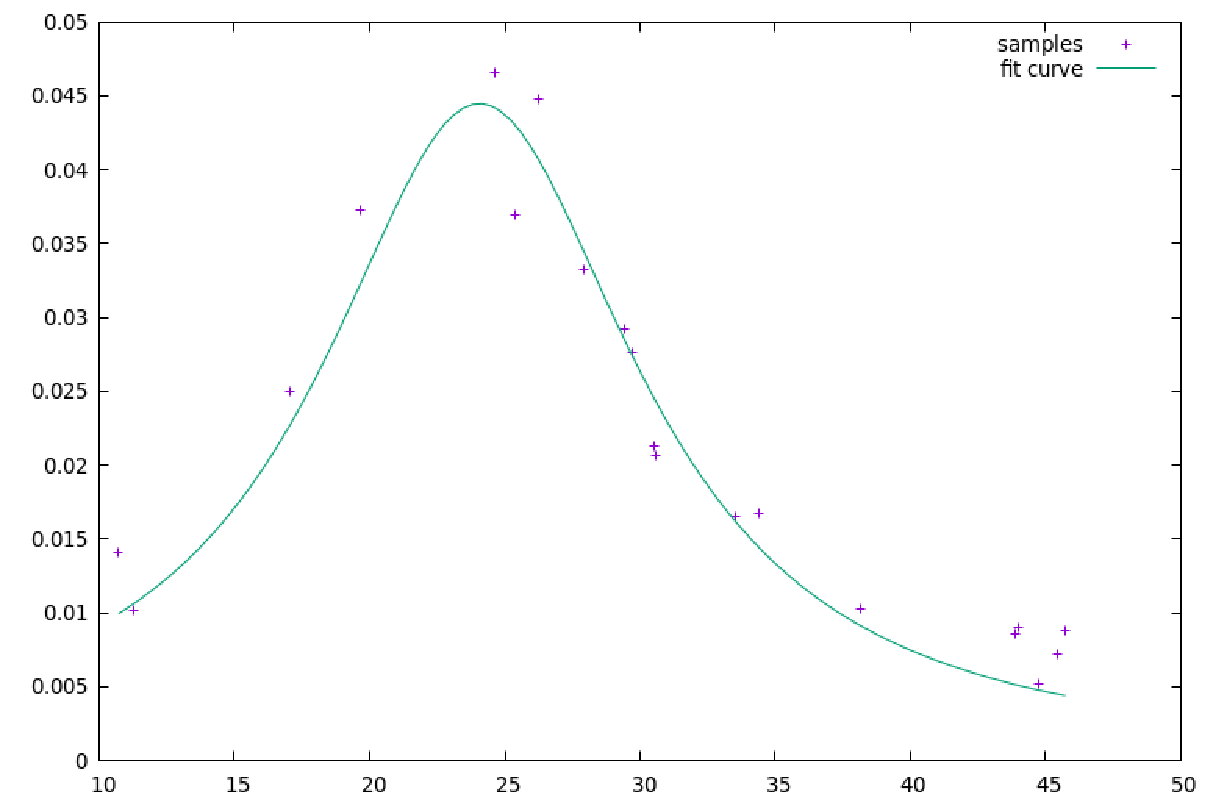
\includegraphics[width=0.7\textwidth]{images/fit_cauchy.pdf}
    \caption{Fitting to a Cauchy distribution}
    \label{fig:example-curve-fitting-cauchy}
\end{figure}

\subsection{Fitting data to a Gaussian distribution}
On adding Gaussian noise of amplitude 0.05 to 50 points sampled from a Gaussian with \\$\mu$ = 2, $\sigma$ = 5, a 
fit is obtained with $\mu$ = 1.95425, $\sigma$ = 4.82169
%$\mu$ = 1.80508, $\sigma$ = 4.85472
\begin{figure}[!ht]
    \centering
    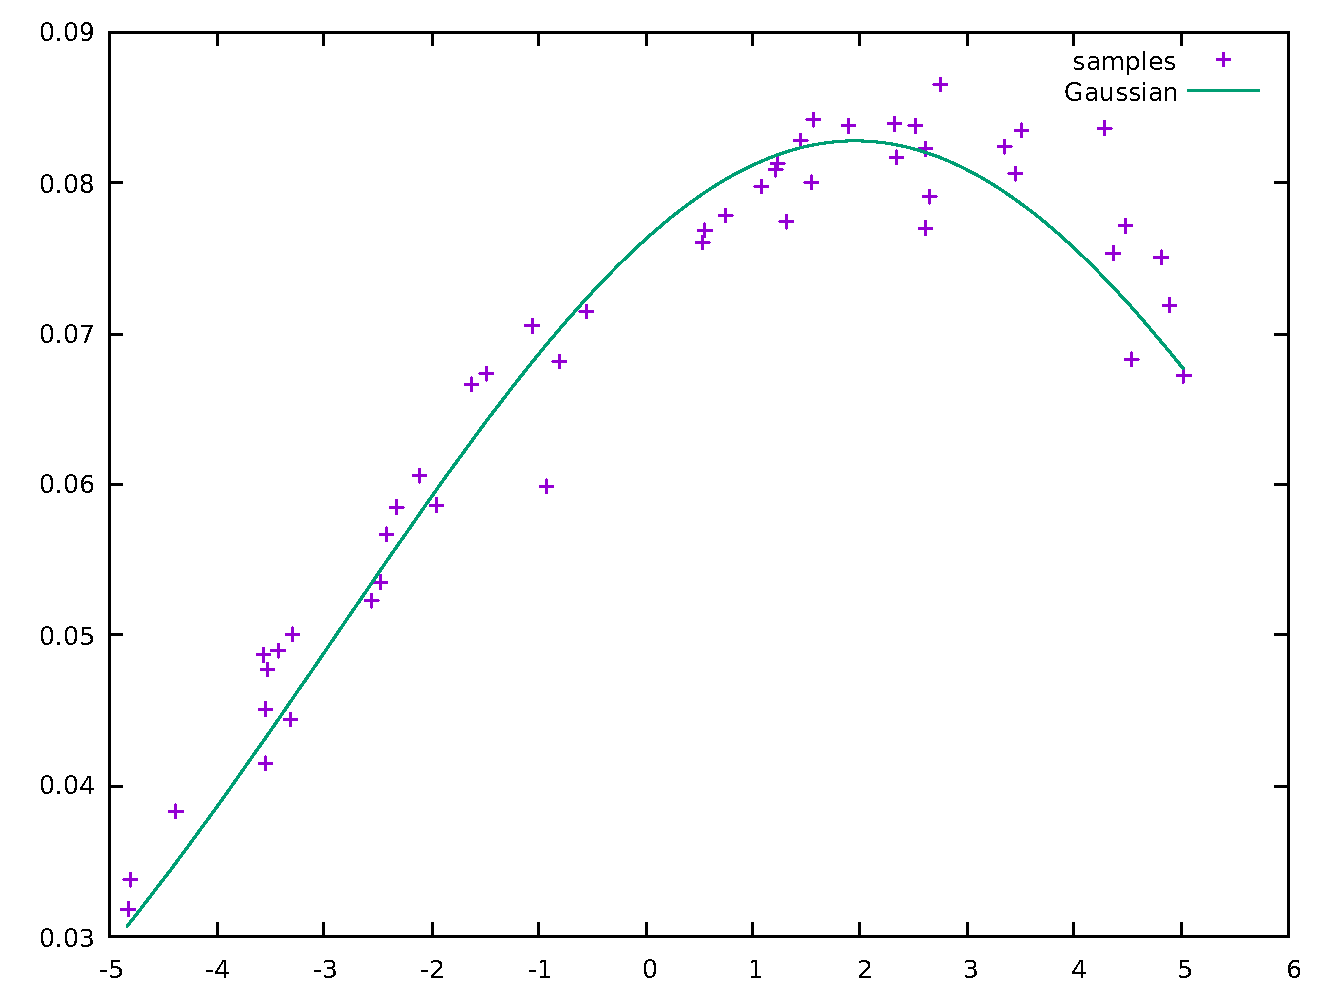
\includegraphics[width=0.7\textwidth]{images/fit_gaussian.pdf}
    \caption{Fitting to a Gaussian distribution}
    \label{fig:example-curve-fitting-gaussian}
\end{figure}

\subsection{\texorpdfstring{Estimating the value of $\pi$ using Monte-Carlo methods}{Estimating the value of pi using Monte-Carlo methods}}
The code for the example can be found under \textit{testing/test\_montecarlo.cpp}
\begin{figure}[!ht]
    \centering
    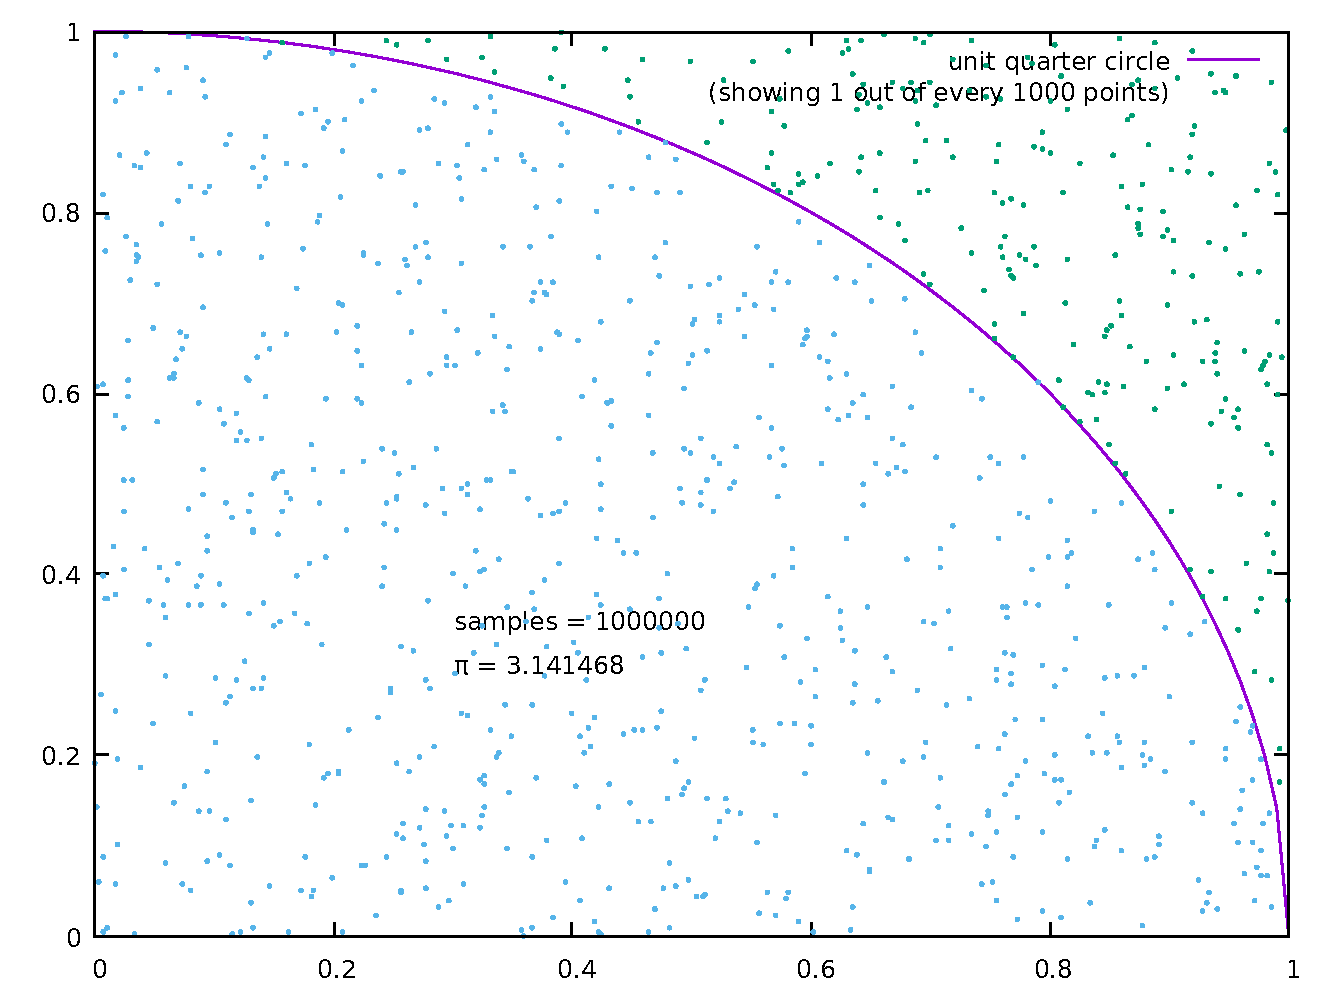
\includegraphics[width=0.7\textwidth]{images/monte_carlo_pi.pdf}
    \caption{Monte-Carlo estimation of $\pi$}
    \label{fig:example-monte-carlo-pi}
\end{figure}

\subsection{Path Tracer using Mersenne Twister to sample BRDFs}
\begin{figure}[!ht]
    \centering
    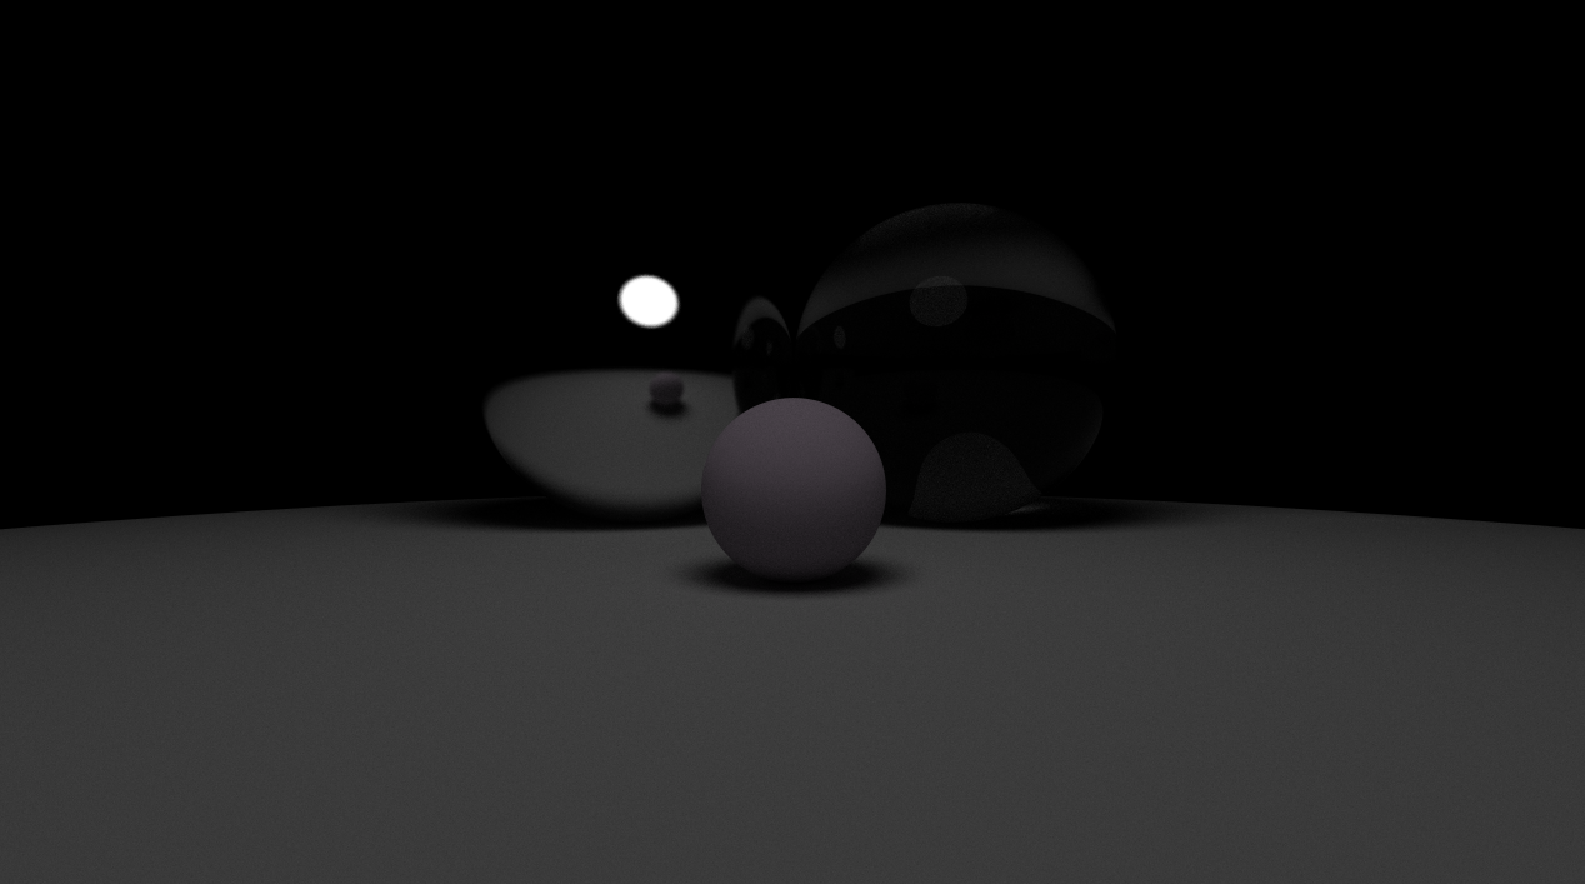
\includegraphics[width=0.7\textwidth]{images/path_tracer.pdf}
    \caption{A Path-Tracer using DiceForge's Mersenne Twister to sample light-ray directions}
    \label{fig:example-path-tracer}
\end{figure}
\newpage
\subsection{Chaos Game using LFSR to choose points}
\begin{figure}[!ht]
    \centering
    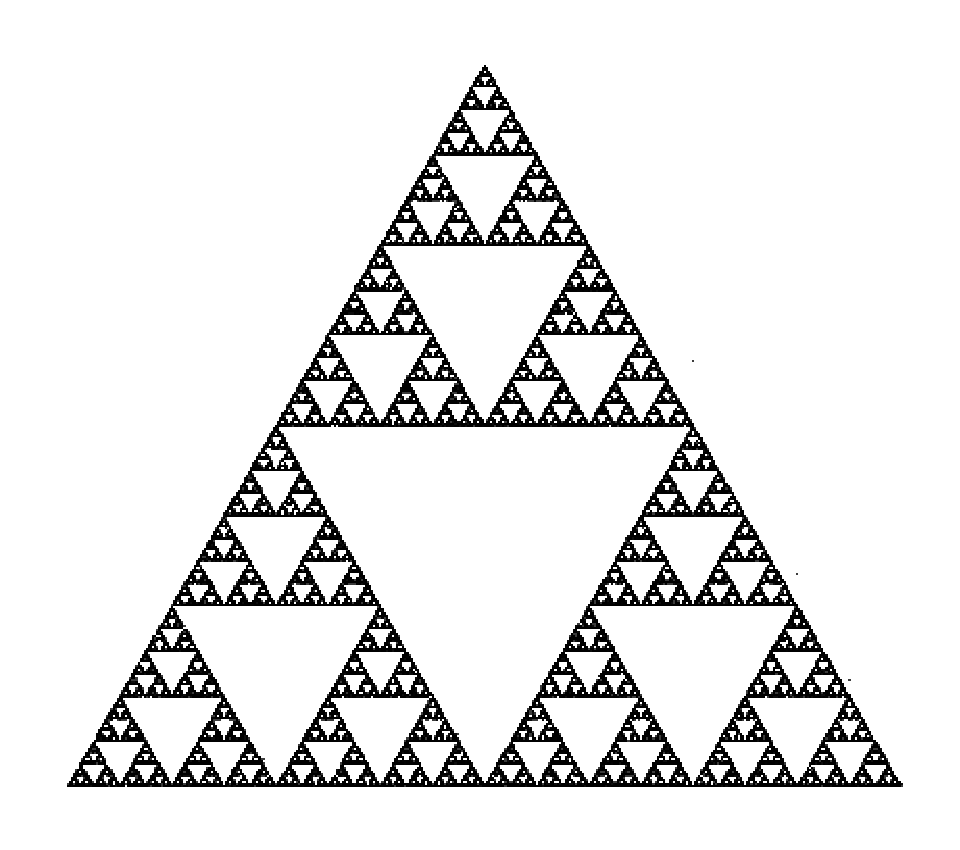
\includegraphics[width=0.7\textwidth]{images/sierpinski_triangle.pdf}
    \caption{A Sierpinski Triangle formed through a Chaos Game using a regular triangle and a factor of $\frac{1}{2}$}
    \label{fig:example-sierpinski-chaos}
\end{figure}

\subsection{Sampling a Maxwell-Boltzmann distribution}
The code for the example can be found under \textit{testing/test\_maxwell.cpp}
\begin{figure}[!ht]
    \centering
    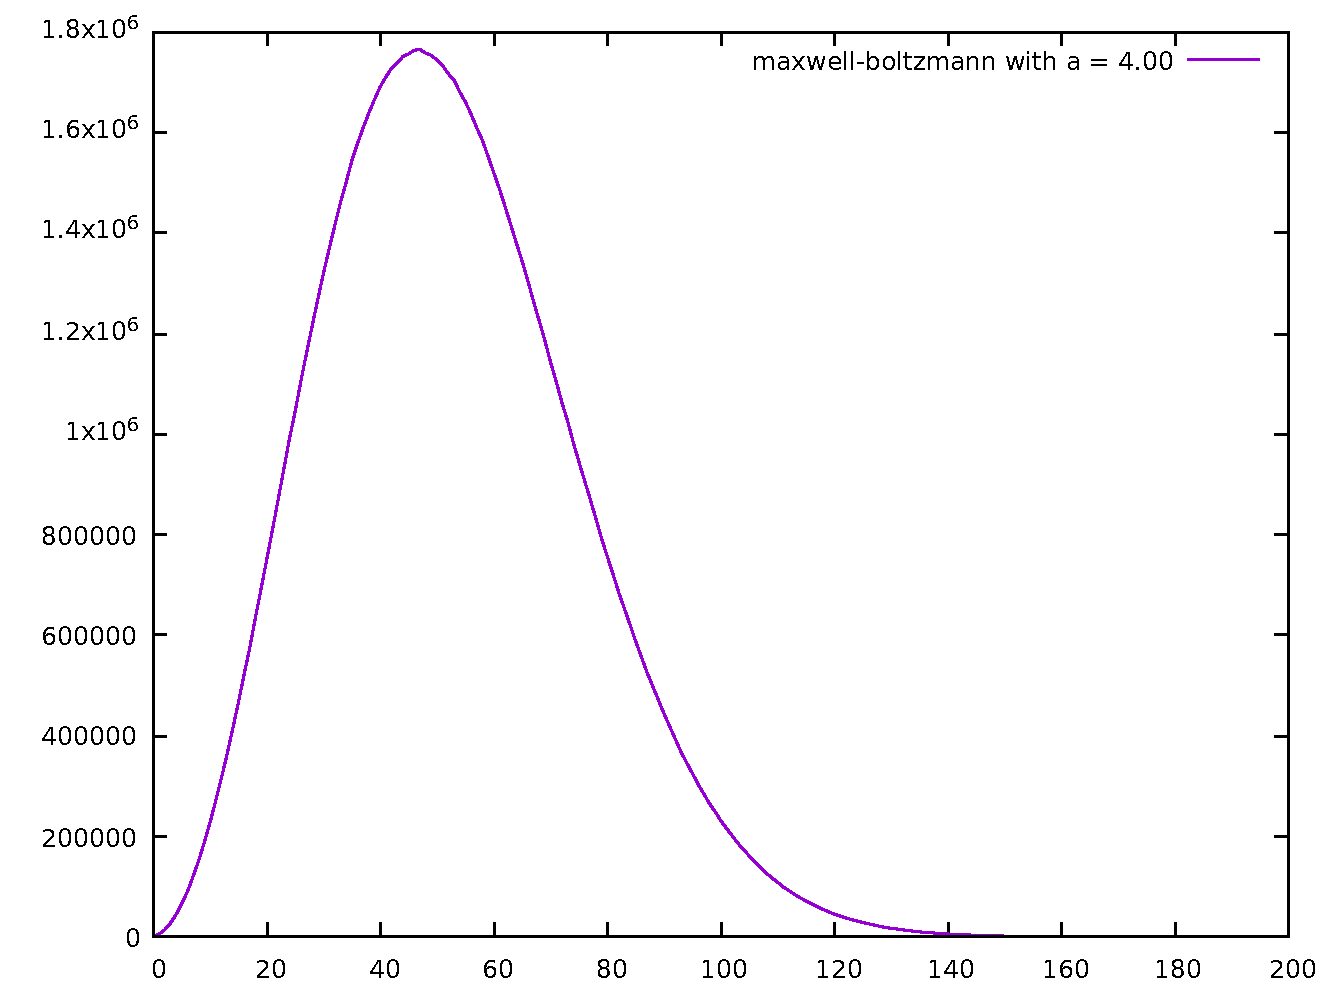
\includegraphics[width=0.7\textwidth]{images/maxwell_pdf.pdf}
    \caption{Histogram of samples from Maxwell-Boltzmann}
    \label{fig:example-sampling-maxwell}
\end{figure}
\newpage
\pagebreak
\section{Appendix}
\subsection{Parameters in Mersenne Twister}
The optimum values for random number generators are :
\newline
32-bit
\begin{itemize}
\item (w,n,m,r)=(32,624,397,31)
\item \textbf{a}= 2573724191
\item \textbf{b}= 0x9d2c5680
\item \textbf{c} = 0xefc60000
\item u  =  11
\item s  =  7
\item t =  15
\item l  = 18
\end{itemize}
64-bit
\begin{itemize}
\item (w,n,m,r)=(64,312,156,31)
\item \textbf{a}= 0xB5026F5AA96619E9
\item \textbf{b}= 0xD66B5EF5B4DA0000
\item \textbf{c} = 0xFDED6BE000000000
\item u  =  29
\item s  =  17
\item t =  37
\item l  = 41
\end{itemize}

\pagebreak

\section{Sources}
\begin{enumerate}
    \item Random Numbers with LFSR (Linear Feedback Shift Register) - Computerphile (\url{https://youtu.be/Ks1pw1X22y4?si=0Wj4uReK7nXS\_OBn})
    \item XORShift RNGs by George Marsaglia (\url{https://www.researchgate.net/publication/5142825_Xorshift_RNGs})
    \item The Dieharder Tests by Robert G. Brown (\url{https://webhome.phy.duke.edu/~rgb/General/dieharder.php})
    \item Integration using Gaussian quadrature\newline
    (\url{https://youtu.be/Hu6yqs0R7GA?si=mztKG7EjKaJvzI5W})
    \item Adaptive Gaussian quadrature 
    (\url{https://youtu.be/U4NUXAwwR8E?si=OwpjGlyJlDe_V1S8})
    \item Non-linear least squares regression (\url{https://www.uio.no/studier/emner/matnat/math/MAT3110/h19/undervisningsmateriale/lecture13.pdf})
    \item Cauchy distributions
    (\url{https://www.itl.nist.gov/div898/handbook/eda/section3/eda3663.htm})
\end{enumerate}
and of course \href{https://www.wikipedia.org/}{Wikipedia}

\end{document}